\documentclass[a4paper]{book}
\usepackage{makeidx}
\usepackage{natbib}
\usepackage{graphicx}
\usepackage{multicol}
\usepackage{float}
\usepackage{listings}
\usepackage{color}
\usepackage{ifthen}
\usepackage[table]{xcolor}
\usepackage{textcomp}
\usepackage{alltt}
\usepackage{ifpdf}
\ifpdf
\usepackage[pdftex,
            pagebackref=true,
            colorlinks=true,
            linkcolor=blue,
            unicode
           ]{hyperref}
\else
\usepackage[ps2pdf,
            pagebackref=true,
            colorlinks=true,
            linkcolor=blue,
            unicode
           ]{hyperref}
\usepackage{pspicture}
\fi
\usepackage[utf8]{inputenc}
\usepackage{mathptmx}
\usepackage[scaled=.90]{helvet}
\usepackage{courier}
\usepackage{sectsty}
\usepackage[titles]{tocloft}
\usepackage{doxygen}
\lstset{language=C++,inputencoding=utf8,basicstyle=\footnotesize,breaklines=true,breakatwhitespace=true,tabsize=8,numbers=left }
\makeindex
\setcounter{tocdepth}{3}
\renewcommand{\footrulewidth}{0.4pt}
\renewcommand{\familydefault}{\sfdefault}
\hfuzz=15pt
\setlength{\emergencystretch}{15pt}
\hbadness=750
\tolerance=750
\begin{document}
\hypersetup{pageanchor=false,citecolor=blue}
\begin{titlepage}
\vspace*{7cm}
\begin{center}
{\Large \-Reference \-Manual}\\
\vspace*{1cm}
{\large \-Generated by Doxygen 1.7.6.1}\\
\vspace*{0.5cm}
{\small Mon Jan 21 2013 16:52:27}\\
\end{center}
\end{titlepage}
\clearemptydoublepage
\pagenumbering{roman}
\tableofcontents
\clearemptydoublepage
\pagenumbering{arabic}
\hypersetup{pageanchor=true,citecolor=blue}
\chapter{\-Class \-Index}
\section{\-Class \-Hierarchy}
\-This inheritance list is sorted roughly, but not completely, alphabetically\-:\begin{DoxyCompactList}
\item \contentsline{section}{\-Ad\-Data}{\pageref{classAdData}}{}
\begin{DoxyCompactList}
\item \contentsline{section}{\-Ad\-Data\-Parallel}{\pageref{classAdDataParallel}}{}
\end{DoxyCompactList}
\item \contentsline{section}{\-Bench}{\pageref{classBench}}{}
\begin{DoxyCompactList}
\item \contentsline{section}{\-Magic\-Square}{\pageref{classMagicSquare}}{}
\end{DoxyCompactList}
\item \contentsline{section}{\-Factory\-Data}{\pageref{classFactoryData}}{}
\begin{DoxyCompactList}
\item \contentsline{section}{\-Factory\-Data\-Par}{\pageref{classFactoryDataPar}}{}
\item \contentsline{section}{\-Factory\-Data\-Seq}{\pageref{classFactoryDataSeq}}{}
\end{DoxyCompactList}
\item \contentsline{section}{\-Strategy\-Cost\-Swap}{\pageref{classStrategyCostSwap}}{}
\begin{DoxyCompactList}
\item \contentsline{section}{\-Default\-Cost\-Swap}{\pageref{classDefaultCostSwap}}{}
\end{DoxyCompactList}
\item \contentsline{section}{\-Strategy\-Cost\-Var}{\pageref{classStrategyCostVar}}{}
\begin{DoxyCompactList}
\item \contentsline{section}{\-Default\-Cost\-Var}{\pageref{classDefaultCostVar}}{}
\end{DoxyCompactList}
\item \contentsline{section}{\-Strategy\-Display\-Sol}{\pageref{classStrategyDisplaySol}}{}
\begin{DoxyCompactList}
\item \contentsline{section}{\-Default\-Display\-Sol}{\pageref{classDefaultDisplaySol}}{}
\end{DoxyCompactList}
\item \contentsline{section}{\-Strategy\-Exec\-Swap}{\pageref{classStrategyExecSwap}}{}
\begin{DoxyCompactList}
\item \contentsline{section}{\-Default\-Exec\-Swap}{\pageref{classDefaultExecSwap}}{}
\end{DoxyCompactList}
\item \contentsline{section}{\-Strategy\-Next\-I}{\pageref{classStrategyNextI}}{}
\begin{DoxyCompactList}
\item \contentsline{section}{\-Default\-Next\-I}{\pageref{classDefaultNextI}}{}
\end{DoxyCompactList}
\item \contentsline{section}{\-Strategy\-Next\-J}{\pageref{classStrategyNextJ}}{}
\begin{DoxyCompactList}
\item \contentsline{section}{\-Default\-Next\-J}{\pageref{classDefaultNextJ}}{}
\end{DoxyCompactList}
\item \contentsline{section}{\-Strategy\-Reset}{\pageref{classStrategyReset}}{}
\begin{DoxyCompactList}
\item \contentsline{section}{\-Default\-Reset}{\pageref{classDefaultReset}}{}
\end{DoxyCompactList}
\item \contentsline{section}{\-Magic\-Square\-:\-:\-X\-Ref}{\pageref{structMagicSquare_1_1XRef}}{}
\end{DoxyCompactList}

\chapter{\-Class \-Index}
\section{\-Class \-List}
\-Here are the classes, structs, unions and interfaces with brief descriptions\-:\begin{DoxyCompactList}
\item\contentsline{section}{\hyperlink{classBench}{\-Bench} \\*\-Benchmark mother class }{\pageref{classBench}}{}
\item\contentsline{section}{\hyperlink{classDefaultCostSwap}{\-Default\-Cost\-Swap} \\*\-Default strategy to compute the cost of a swap }{\pageref{classDefaultCostSwap}}{}
\item\contentsline{section}{\hyperlink{classDefaultCostVar}{\-Default\-Cost\-Var} \\*\-Default strategy to compute the cost of a swap }{\pageref{classDefaultCostVar}}{}
\item\contentsline{section}{\hyperlink{classDefaultDisplaySol}{\-Default\-Display\-Sol} \\*\-Default strategy to display the solution }{\pageref{classDefaultDisplaySol}}{}
\item\contentsline{section}{\hyperlink{classDefaultExecSwap}{\-Default\-Exec\-Swap} \\*\-Default strategy to execute a swap }{\pageref{classDefaultExecSwap}}{}
\item\contentsline{section}{\hyperlink{classDefaultNextI}{\-Default\-Next\-I} \\*\-Default strategy to return the next i (variable) to consider }{\pageref{classDefaultNextI}}{}
\item\contentsline{section}{\hyperlink{classDefaultNextJ}{\-Default\-Next\-J} \\*\-Default strategy to return the next j (value) to consider, given i (variable) }{\pageref{classDefaultNextJ}}{}
\item\contentsline{section}{\hyperlink{classDefaultReset}{\-Default\-Reset} \\*\-Default strategy to perform a reset }{\pageref{classDefaultReset}}{}
\item\contentsline{section}{\hyperlink{classMagicSquare}{\-Magic\-Square} }{\pageref{classMagicSquare}}{}
\item\contentsline{section}{\hyperlink{classStrategyCostSwap}{\-Strategy\-Cost\-Swap} \\*\-Strategy \-Pattern to compute the cost of a swap }{\pageref{classStrategyCostSwap}}{}
\item\contentsline{section}{\hyperlink{classStrategyCostVar}{\-Strategy\-Cost\-Var} \\*\-Strategy \-Pattern to compute the projected cost on a variable }{\pageref{classStrategyCostVar}}{}
\item\contentsline{section}{\hyperlink{classStrategyDisplaySol}{\-Strategy\-Display\-Sol} \\*\-Strategy \-Pattern to display the solution }{\pageref{classStrategyDisplaySol}}{}
\item\contentsline{section}{\hyperlink{classStrategyExecSwap}{\-Strategy\-Exec\-Swap} \\*\-Strategy \-Pattern to execute a swap }{\pageref{classStrategyExecSwap}}{}
\item\contentsline{section}{\hyperlink{classStrategyNextI}{\-Strategy\-Next\-I} \\*\-Strategy \-Pattern to return the next i (variable) to consider }{\pageref{classStrategyNextI}}{}
\item\contentsline{section}{\hyperlink{classStrategyNextJ}{\-Strategy\-Next\-J} \\*\-Strategy \-Pattern to return the next j (value) to consider, given i (variable) }{\pageref{classStrategyNextJ}}{}
\item\contentsline{section}{\hyperlink{classStrategyReset}{\-Strategy\-Reset} \\*\-Strategy \-Pattern to perform a reset }{\pageref{classStrategyReset}}{}
\item\contentsline{section}{\hyperlink{structMagicSquare_1_1XRef}{\-Magic\-Square\-::\-X\-Ref} }{\pageref{structMagicSquare_1_1XRef}}{}
\end{DoxyCompactList}

\chapter{\-File \-Index}
\section{File List}
Here is a list of all documented files with brief descriptions:\begin{DoxyCompactList}
\item\contentsline{section}{\hyperlink{bench_8cpp}{bench.cpp} (Benchmark mother class )}{\pageref{bench_8cpp}}{}
\item\contentsline{section}{\hyperlink{bench_8h}{bench.h} (Benchmark mother class )}{\pageref{bench_8h}}{}
\item\contentsline{section}{\hyperlink{magic__square_8cpp}{magic\_\-square.cpp} (Magic Square benchmark )}{\pageref{magic__square_8cpp}}{}
\item\contentsline{section}{\hyperlink{magic__square_8h}{magic\_\-square.h} (Magic Square benchmark )}{\pageref{magic__square_8h}}{}
\end{DoxyCompactList}

\chapter{\-Class \-Documentation}
\hypertarget{classBench}{\section{\-Bench \-Class \-Reference}
\label{classBench}\index{\-Bench@{\-Bench}}
}


\-Benchmark mother class.  




{\ttfamily \#include $<$bench.\-hpp$>$}

\-Inheritance diagram for \-Bench\-:\begin{figure}[H]
\begin{center}
\leavevmode
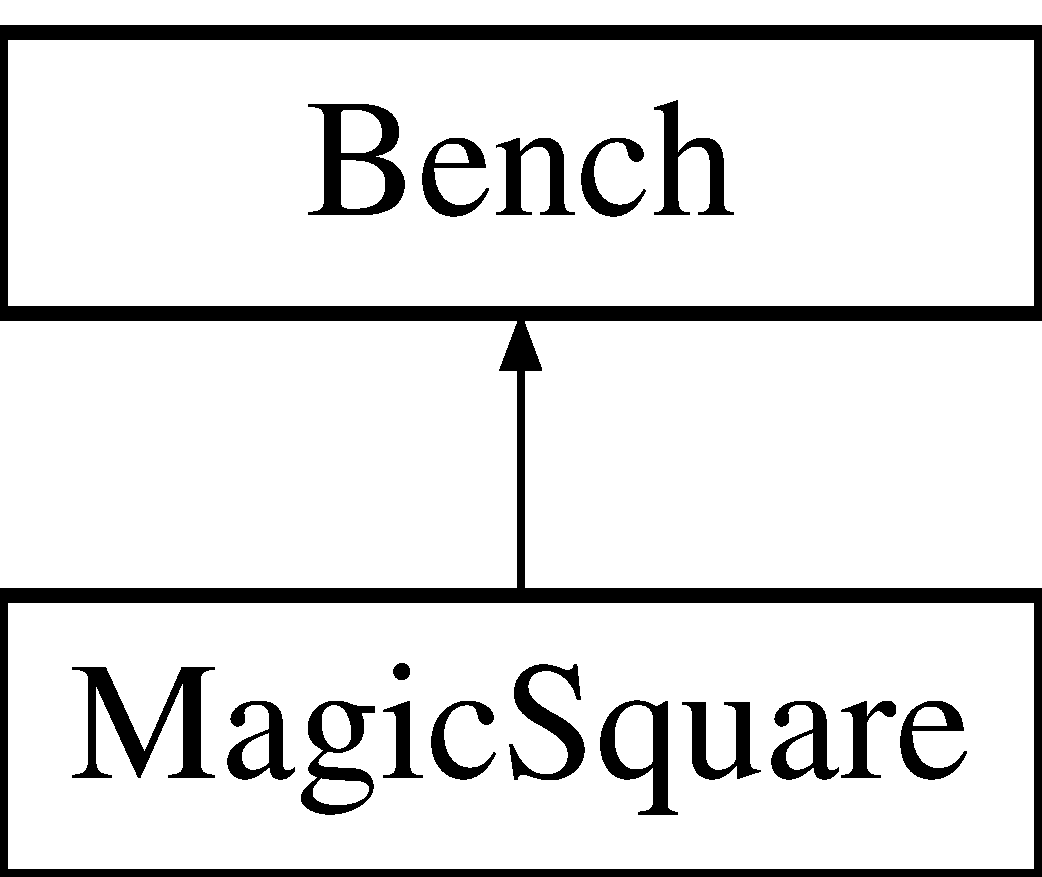
\includegraphics[height=2.000000cm]{classBench}
\end{center}
\end{figure}
\subsection*{\-Public \-Member \-Functions}
\begin{DoxyCompactItemize}
\item 
int \hyperlink{classBench_a5d88ce438e5ff9259f872bdcfe86621e}{cost\-If\-Swap} (int current\-Cost, int i, int j)
\begin{DoxyCompactList}\small\item\em \-Wrapper when user function cost\-If\-Swap is not defined. \end{DoxyCompactList}\item 
int \hyperlink{classBench_af27d153047259b80af7b556c0bfdadab}{cost\-On\-Variable} (int k)
\begin{DoxyCompactList}\small\item\em \-Wrapper when user function cost\-On\-Variable is not defined. \end{DoxyCompactList}\item 
void \hyperlink{classBench_a8f1d5b7a37082ec2f2bb15b9e3820c96}{display\-Solution} (\hyperlink{classAdData}{\-Ad\-Data} $\ast$p\-\_\-ad)
\begin{DoxyCompactList}\small\item\em \-Wrapper when user function display\-Solution is not defined. \end{DoxyCompactList}\item 
void \hyperlink{classBench_a0985e6c65a50742c898dd717dce2294c}{executed\-Swap} (int k1, int k2)
\begin{DoxyCompactList}\small\item\em \-Wrapper when user function executed\-Swap is not defined. \end{DoxyCompactList}\item 
int \hyperlink{classBench_a2ace948d46b3bcc7d76b2a4a32b427cd}{next\-I} (int i)
\begin{DoxyCompactList}\small\item\em \-Wrapper when user function next\-I is not defined. \end{DoxyCompactList}\item 
int \hyperlink{classBench_a5bc8976d21762350873d32e5f64a8d70}{next\-J} (int i, int j)
\begin{DoxyCompactList}\small\item\em \-Wrapper when user function next\-J is not defined. \end{DoxyCompactList}\item 
int \hyperlink{classBench_a0a317019a5065efe4bc37d1760379786}{reset} (int n, \hyperlink{classAdData}{\-Ad\-Data} $\ast$p\-\_\-ad)
\begin{DoxyCompactList}\small\item\em \-Wrapper when user function reset is not defined. \end{DoxyCompactList}\end{DoxyCompactItemize}
\subsection*{\-Public \-Attributes}
\begin{DoxyCompactItemize}
\item 
\hyperlink{classStrategyCostSwap}{\-Strategy\-Cost\-Swap} \hyperlink{classBench_a27ed9ea3eb2b29027e79e31adf331d86}{strategy\-Cost\-Swap}
\item 
\hyperlink{classStrategyCostVar}{\-Strategy\-Cost\-Var} \hyperlink{classBench_a2ce57cda8198f6be72fd0ac045b06839}{strategy\-Cost\-Var}
\item 
\hyperlink{classStrategyDisplaySol}{\-Strategy\-Display\-Sol} \hyperlink{classBench_a31569ae22eda31c68257050276fa6fee}{strategy\-Display\-Sol}
\item 
\hyperlink{classStrategyExecSwap}{\-Strategy\-Exec\-Swap} \hyperlink{classBench_a8737cee0eb80295048068322c9a20359}{strategy\-Exec\-Swap}
\item 
\hyperlink{classStrategyNextI}{\-Strategy\-Next\-I} \hyperlink{classBench_af15b42b6084454f59cd63cf9968a2a5b}{strategy\-Next\-I}
\item 
\hyperlink{classStrategyNextJ}{\-Strategy\-Next\-J} \hyperlink{classBench_a4a1797a7ffaa0ce346274ac63f2379b3}{strategy\-Next\-J}
\item 
\hyperlink{classStrategyReset}{\-Strategy\-Reset} \hyperlink{classBench_a88dbf079cc6c2392132efc8038b88443}{strategy\-Reset}
\end{DoxyCompactItemize}


\subsection{\-Detailed \-Description}
\-Benchmark mother class. 

\subsection{\-Member \-Function \-Documentation}
\hypertarget{classBench_a5d88ce438e5ff9259f872bdcfe86621e}{\index{\-Bench@{\-Bench}!cost\-If\-Swap@{cost\-If\-Swap}}
\index{cost\-If\-Swap@{cost\-If\-Swap}!Bench@{\-Bench}}
\subsubsection[{cost\-If\-Swap}]{\setlength{\rightskip}{0pt plus 5cm}int {\bf \-Bench\-::cost\-If\-Swap} (
\begin{DoxyParamCaption}
\item[{int}]{current\-Cost, }
\item[{int}]{i, }
\item[{int}]{j}
\end{DoxyParamCaption}
)}}\label{classBench_a5d88ce438e5ff9259f872bdcfe86621e}


\-Wrapper when user function cost\-If\-Swap is not defined. 


\begin{DoxyParams}{\-Parameters}
{\em current\-Cost,\-:} & the current cost when this function is called. i and j, the variables with which we simulate a swap to compute the resulting cost. \\
\hline
\end{DoxyParams}
\begin{DoxyReturn}{\-Returns}
\-The cost if we swap variables i and j. 
\end{DoxyReturn}


\-Reimplemented in \hyperlink{classMagicSquare_a3904934cb8ef871455a57dd0dd9be7ea}{\-Magic\-Square}.

\hypertarget{classBench_af27d153047259b80af7b556c0bfdadab}{\index{\-Bench@{\-Bench}!cost\-On\-Variable@{cost\-On\-Variable}}
\index{cost\-On\-Variable@{cost\-On\-Variable}!Bench@{\-Bench}}
\subsubsection[{cost\-On\-Variable}]{\setlength{\rightskip}{0pt plus 5cm}int {\bf \-Bench\-::cost\-On\-Variable} (
\begin{DoxyParamCaption}
\item[{int}]{k}
\end{DoxyParamCaption}
)}}\label{classBench_af27d153047259b80af7b556c0bfdadab}


\-Wrapper when user function cost\-On\-Variable is not defined. 


\begin{DoxyParams}{\-Parameters}
{\em k,\-:} & the variable on which we project the cost. \\
\hline
\end{DoxyParams}
\begin{DoxyReturn}{\-Returns}
\-The cost projected on variable k. 
\end{DoxyReturn}


\-Reimplemented in \hyperlink{classMagicSquare_ae57a2b1183f82870cdd63fddeeb078fe}{\-Magic\-Square}.

\hypertarget{classBench_a8f1d5b7a37082ec2f2bb15b9e3820c96}{\index{\-Bench@{\-Bench}!display\-Solution@{display\-Solution}}
\index{display\-Solution@{display\-Solution}!Bench@{\-Bench}}
\subsubsection[{display\-Solution}]{\setlength{\rightskip}{0pt plus 5cm}void {\bf \-Bench\-::display\-Solution} (
\begin{DoxyParamCaption}
\item[{{\bf \-Ad\-Data} $\ast$}]{p\-\_\-ad}
\end{DoxyParamCaption}
)}}\label{classBench_a8f1d5b7a37082ec2f2bb15b9e3820c96}


\-Wrapper when user function display\-Solution is not defined. 


\begin{DoxyParams}{\-Parameters}
{\em p\-\_\-ad,\-:} & \-Pointer toward the current configuration (or solution). \\
\hline
\end{DoxyParams}
\hypertarget{classBench_a0985e6c65a50742c898dd717dce2294c}{\index{\-Bench@{\-Bench}!executed\-Swap@{executed\-Swap}}
\index{executed\-Swap@{executed\-Swap}!Bench@{\-Bench}}
\subsubsection[{executed\-Swap}]{\setlength{\rightskip}{0pt plus 5cm}void {\bf \-Bench\-::executed\-Swap} (
\begin{DoxyParamCaption}
\item[{int}]{k1, }
\item[{int}]{k2}
\end{DoxyParamCaption}
)}}\label{classBench_a0985e6c65a50742c898dd717dce2294c}


\-Wrapper when user function executed\-Swap is not defined. 


\begin{DoxyParams}{\-Parameters}
{\em k1} & and k2\-: variables to swap. \\
\hline
\end{DoxyParams}


\-Reimplemented in \hyperlink{classMagicSquare_a63c7d1ad48a11ff2e2b1889ae883cc0d}{\-Magic\-Square}.

\hypertarget{classBench_a2ace948d46b3bcc7d76b2a4a32b427cd}{\index{\-Bench@{\-Bench}!next\-I@{next\-I}}
\index{next\-I@{next\-I}!Bench@{\-Bench}}
\subsubsection[{next\-I}]{\setlength{\rightskip}{0pt plus 5cm}int {\bf \-Bench\-::next\-I} (
\begin{DoxyParamCaption}
\item[{int}]{i}
\end{DoxyParamCaption}
)}}\label{classBench_a2ace948d46b3bcc7d76b2a4a32b427cd}


\-Wrapper when user function next\-I is not defined. 


\begin{DoxyParams}{\-Parameters}
{\em i,\-:} & a variable. \\
\hline
\end{DoxyParams}
\begin{DoxyReturn}{\-Returns}
\-The next variable (i+1) 
\end{DoxyReturn}
\hypertarget{classBench_a5bc8976d21762350873d32e5f64a8d70}{\index{\-Bench@{\-Bench}!next\-J@{next\-J}}
\index{next\-J@{next\-J}!Bench@{\-Bench}}
\subsubsection[{next\-J}]{\setlength{\rightskip}{0pt plus 5cm}int {\bf \-Bench\-::next\-J} (
\begin{DoxyParamCaption}
\item[{int}]{i, }
\item[{int}]{j}
\end{DoxyParamCaption}
)}}\label{classBench_a5bc8976d21762350873d32e5f64a8d70}


\-Wrapper when user function next\-J is not defined. 


\begin{DoxyParams}{\-Parameters}
{\em i} & and j\-: two variables. \\
\hline
\end{DoxyParams}
\begin{DoxyReturn}{\-Returns}
\-The next j-\/variable (j+1), unless j $<$ 0 (then returns i+1) 
\end{DoxyReturn}
\hypertarget{classBench_a0a317019a5065efe4bc37d1760379786}{\index{\-Bench@{\-Bench}!reset@{reset}}
\index{reset@{reset}!Bench@{\-Bench}}
\subsubsection[{reset}]{\setlength{\rightskip}{0pt plus 5cm}int {\bf \-Bench\-::reset} (
\begin{DoxyParamCaption}
\item[{int}]{n, }
\item[{{\bf \-Ad\-Data} $\ast$}]{p\-\_\-ad}
\end{DoxyParamCaption}
)}}\label{classBench_a0a317019a5065efe4bc37d1760379786}


\-Wrapper when user function reset is not defined. 


\begin{DoxyParams}{\-Parameters}
{\em n,\-:} & number of reset loop to perform. p\-\_\-ad\-: pointer toward the configuration. \\
\hline
\end{DoxyParams}
\begin{DoxyReturn}{\-Returns}
\-The new cost, or -\/1 if unknown. 
\end{DoxyReturn}


\subsection{\-Member \-Data \-Documentation}
\hypertarget{classBench_a27ed9ea3eb2b29027e79e31adf331d86}{\index{\-Bench@{\-Bench}!strategy\-Cost\-Swap@{strategy\-Cost\-Swap}}
\index{strategy\-Cost\-Swap@{strategy\-Cost\-Swap}!Bench@{\-Bench}}
\subsubsection[{strategy\-Cost\-Swap}]{\setlength{\rightskip}{0pt plus 5cm}{\bf \-Strategy\-Cost\-Swap} {\bf \-Bench\-::strategy\-Cost\-Swap}}}\label{classBench_a27ed9ea3eb2b29027e79e31adf331d86}
\-Stragety \-Pattern to compute the cost of a swap \hypertarget{classBench_a2ce57cda8198f6be72fd0ac045b06839}{\index{\-Bench@{\-Bench}!strategy\-Cost\-Var@{strategy\-Cost\-Var}}
\index{strategy\-Cost\-Var@{strategy\-Cost\-Var}!Bench@{\-Bench}}
\subsubsection[{strategy\-Cost\-Var}]{\setlength{\rightskip}{0pt plus 5cm}{\bf \-Strategy\-Cost\-Var} {\bf \-Bench\-::strategy\-Cost\-Var}}}\label{classBench_a2ce57cda8198f6be72fd0ac045b06839}
\-Stragety \-Pattern to compute the projected cost on a variable \hypertarget{classBench_a31569ae22eda31c68257050276fa6fee}{\index{\-Bench@{\-Bench}!strategy\-Display\-Sol@{strategy\-Display\-Sol}}
\index{strategy\-Display\-Sol@{strategy\-Display\-Sol}!Bench@{\-Bench}}
\subsubsection[{strategy\-Display\-Sol}]{\setlength{\rightskip}{0pt plus 5cm}{\bf \-Strategy\-Display\-Sol} {\bf \-Bench\-::strategy\-Display\-Sol}}}\label{classBench_a31569ae22eda31c68257050276fa6fee}
\-Stragety \-Pattern to display the solution \hypertarget{classBench_a8737cee0eb80295048068322c9a20359}{\index{\-Bench@{\-Bench}!strategy\-Exec\-Swap@{strategy\-Exec\-Swap}}
\index{strategy\-Exec\-Swap@{strategy\-Exec\-Swap}!Bench@{\-Bench}}
\subsubsection[{strategy\-Exec\-Swap}]{\setlength{\rightskip}{0pt plus 5cm}{\bf \-Strategy\-Exec\-Swap} {\bf \-Bench\-::strategy\-Exec\-Swap}}}\label{classBench_a8737cee0eb80295048068322c9a20359}
\-Stragety \-Pattern to execute a swap \hypertarget{classBench_af15b42b6084454f59cd63cf9968a2a5b}{\index{\-Bench@{\-Bench}!strategy\-Next\-I@{strategy\-Next\-I}}
\index{strategy\-Next\-I@{strategy\-Next\-I}!Bench@{\-Bench}}
\subsubsection[{strategy\-Next\-I}]{\setlength{\rightskip}{0pt plus 5cm}{\bf \-Strategy\-Next\-I} {\bf \-Bench\-::strategy\-Next\-I}}}\label{classBench_af15b42b6084454f59cd63cf9968a2a5b}
\-Stragety \-Pattern to return the next i (variable) to consider \hypertarget{classBench_a4a1797a7ffaa0ce346274ac63f2379b3}{\index{\-Bench@{\-Bench}!strategy\-Next\-J@{strategy\-Next\-J}}
\index{strategy\-Next\-J@{strategy\-Next\-J}!Bench@{\-Bench}}
\subsubsection[{strategy\-Next\-J}]{\setlength{\rightskip}{0pt plus 5cm}{\bf \-Strategy\-Next\-J} {\bf \-Bench\-::strategy\-Next\-J}}}\label{classBench_a4a1797a7ffaa0ce346274ac63f2379b3}
\-Stragety \-Pattern to return the next j (value) to consider, given i (variable) \hypertarget{classBench_a88dbf079cc6c2392132efc8038b88443}{\index{\-Bench@{\-Bench}!strategy\-Reset@{strategy\-Reset}}
\index{strategy\-Reset@{strategy\-Reset}!Bench@{\-Bench}}
\subsubsection[{strategy\-Reset}]{\setlength{\rightskip}{0pt plus 5cm}{\bf \-Strategy\-Reset} {\bf \-Bench\-::strategy\-Reset}}}\label{classBench_a88dbf079cc6c2392132efc8038b88443}
\-Stragety \-Pattern to perform a reset 

\-The documentation for this class was generated from the following files\-:\begin{DoxyCompactItemize}
\item 
include/\hyperlink{bench_8hpp}{bench.\-hpp}\item 
src/\hyperlink{bench_8cpp}{bench.\-cpp}\end{DoxyCompactItemize}

\hypertarget{classDefaultCostSwap}{\section{\-Default\-Cost\-Swap \-Class \-Reference}
\label{classDefaultCostSwap}\index{\-Default\-Cost\-Swap@{\-Default\-Cost\-Swap}}
}


\-Default strategy to compute the cost of a swap.  




{\ttfamily \#include $<$default\-\_\-cost\-\_\-swap.\-hpp$>$}

\-Inheritance diagram for \-Default\-Cost\-Swap\-:\begin{figure}[H]
\begin{center}
\leavevmode
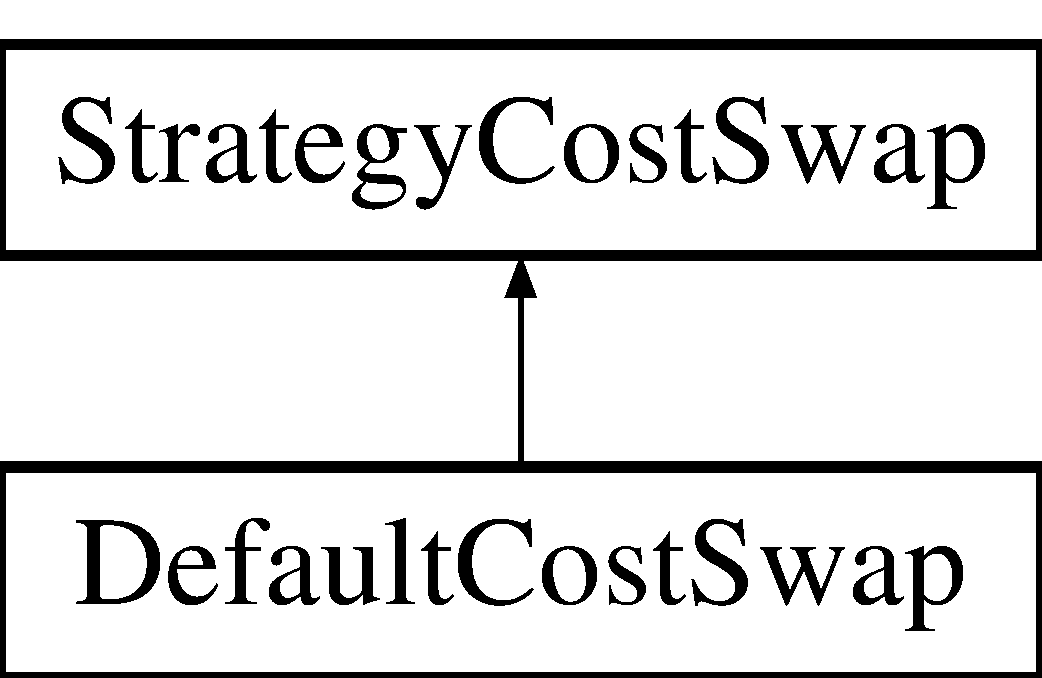
\includegraphics[height=2.000000cm]{classDefaultCostSwap}
\end{center}
\end{figure}
\subsection*{\-Public \-Member \-Functions}
\begin{DoxyCompactItemize}
\item 
int \hyperlink{classDefaultCostSwap_a62c43925fb3f931b12f92d3a1bbfc55f}{cost\-If\-Swap} (int current\-Cost, int i, int j)
\begin{DoxyCompactList}\small\item\em \-Wrapper when user function cost\-If\-Swap is not defined. \end{DoxyCompactList}\end{DoxyCompactItemize}


\subsection{\-Detailed \-Description}
\-Default strategy to compute the cost of a swap. 

\subsection{\-Member \-Function \-Documentation}
\hypertarget{classDefaultCostSwap_a62c43925fb3f931b12f92d3a1bbfc55f}{\index{\-Default\-Cost\-Swap@{\-Default\-Cost\-Swap}!cost\-If\-Swap@{cost\-If\-Swap}}
\index{cost\-If\-Swap@{cost\-If\-Swap}!DefaultCostSwap@{\-Default\-Cost\-Swap}}
\subsubsection[{cost\-If\-Swap}]{\setlength{\rightskip}{0pt plus 5cm}int {\bf \-Default\-Cost\-Swap\-::cost\-If\-Swap} (
\begin{DoxyParamCaption}
\item[{int}]{current\-Cost, }
\item[{int}]{i, }
\item[{int}]{j}
\end{DoxyParamCaption}
)\hspace{0.3cm}{\ttfamily  \mbox{[}virtual\mbox{]}}}}\label{classDefaultCostSwap_a62c43925fb3f931b12f92d3a1bbfc55f}


\-Wrapper when user function cost\-If\-Swap is not defined. 


\begin{DoxyParams}{\-Parameters}
{\em current\-Cost,\-:} & the current cost when this function is called. i and j, the variables with which we simulate a swap to compute the resulting cost. \\
\hline
\end{DoxyParams}
\begin{DoxyReturn}{\-Returns}
\-The cost if we swap variables i and j. 
\end{DoxyReturn}


\-Implements \hyperlink{classStrategyCostSwap_a154e8db5c0e7cc22bd33942bbe4b8618}{\-Strategy\-Cost\-Swap}.



\-The documentation for this class was generated from the following files\-:\begin{DoxyCompactItemize}
\item 
include/\hyperlink{default__cost__swap_8hpp}{default\-\_\-cost\-\_\-swap.\-hpp}\item 
src/\hyperlink{default__cost__swap_8cpp}{default\-\_\-cost\-\_\-swap.\-cpp}\end{DoxyCompactItemize}

\hypertarget{classDefaultCostVar}{\section{\-Default\-Cost\-Var \-Class \-Reference}
\label{classDefaultCostVar}\index{\-Default\-Cost\-Var@{\-Default\-Cost\-Var}}
}


\-Default strategy to compute the cost of a swap.  




{\ttfamily \#include $<$default\-\_\-cost\-\_\-var.\-h$>$}

\-Inheritance diagram for \-Default\-Cost\-Var\-:\begin{figure}[H]
\begin{center}
\leavevmode
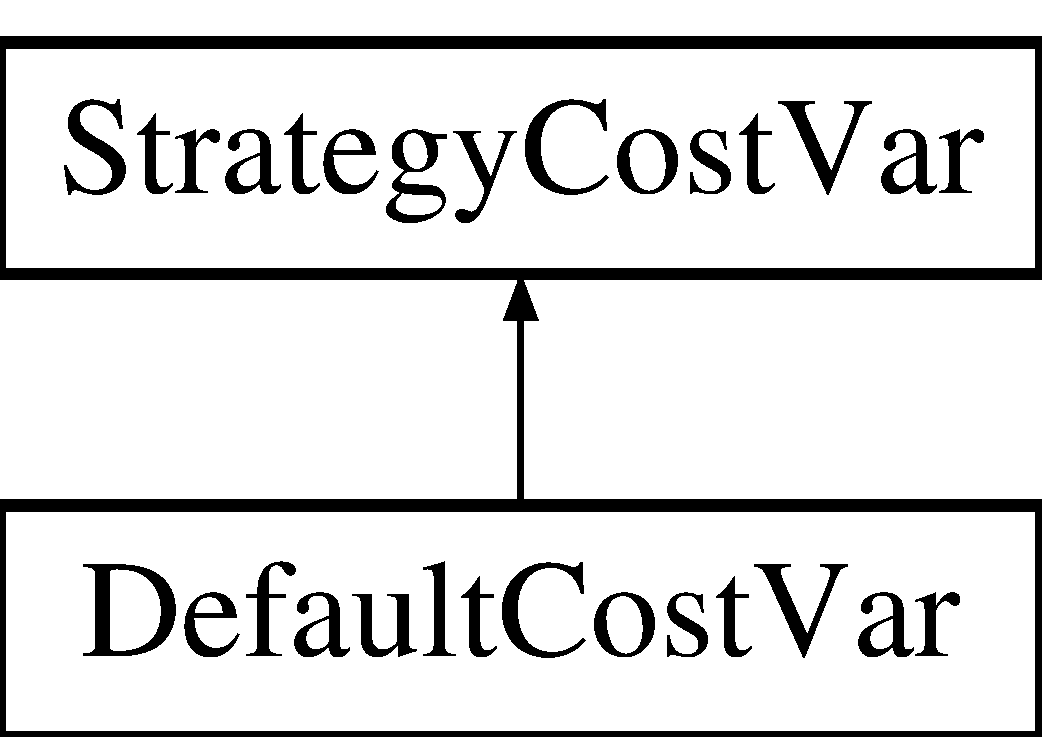
\includegraphics[height=2.000000cm]{classDefaultCostVar}
\end{center}
\end{figure}
\subsection*{\-Public \-Member \-Functions}
\begin{DoxyCompactItemize}
\item 
int \hyperlink{classDefaultCostVar_a24820c1212f4e6f686156e9c0d3f2795}{cost\-On\-Variable} (int k)
\begin{DoxyCompactList}\small\item\em \-Virtual wrapper when user function cost\-On\-Variable is not defined. \end{DoxyCompactList}\end{DoxyCompactItemize}


\subsection{\-Detailed \-Description}
\-Default strategy to compute the cost of a swap. 

\subsection{\-Member \-Function \-Documentation}
\hypertarget{classDefaultCostVar_a24820c1212f4e6f686156e9c0d3f2795}{\index{\-Default\-Cost\-Var@{\-Default\-Cost\-Var}!cost\-On\-Variable@{cost\-On\-Variable}}
\index{cost\-On\-Variable@{cost\-On\-Variable}!DefaultCostVar@{\-Default\-Cost\-Var}}
\subsubsection[{cost\-On\-Variable}]{\setlength{\rightskip}{0pt plus 5cm}int {\bf \-Default\-Cost\-Var\-::cost\-On\-Variable} (
\begin{DoxyParamCaption}
\item[{int}]{k}
\end{DoxyParamCaption}
)\hspace{0.3cm}{\ttfamily  \mbox{[}inline, virtual\mbox{]}}}}\label{classDefaultCostVar_a24820c1212f4e6f686156e9c0d3f2795}


\-Virtual wrapper when user function cost\-On\-Variable is not defined. 


\begin{DoxyParams}{\-Parameters}
{\em k,\-:} & the variable on which we project the cost. \\
\hline
\end{DoxyParams}
\begin{DoxyReturn}{\-Returns}
\-The cost projected on variable k. 
\end{DoxyReturn}


\-Implements \hyperlink{classStrategyCostVar_a8381829dfa84b3460822aa0e3677a443}{\-Strategy\-Cost\-Var}.



\-The documentation for this class was generated from the following file\-:\begin{DoxyCompactItemize}
\item 
\hyperlink{default__cost__var_8h}{default\-\_\-cost\-\_\-var.\-h}\end{DoxyCompactItemize}

\hypertarget{classDefaultDisplaySol}{\section{\-Default\-Display\-Sol \-Class \-Reference}
\label{classDefaultDisplaySol}\index{\-Default\-Display\-Sol@{\-Default\-Display\-Sol}}
}


\-Default strategy to display the solution.  




{\ttfamily \#include $<$default\-\_\-display\-\_\-sol.\-hpp$>$}

\-Inheritance diagram for \-Default\-Display\-Sol\-:\begin{figure}[H]
\begin{center}
\leavevmode
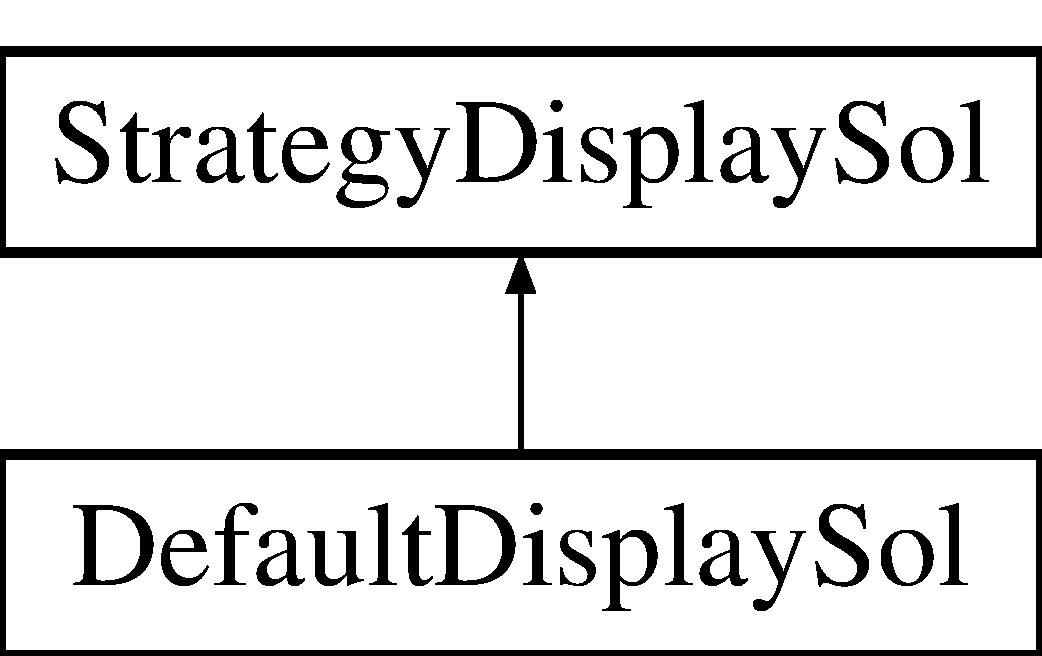
\includegraphics[height=2.000000cm]{classDefaultDisplaySol}
\end{center}
\end{figure}
\subsection*{\-Public \-Member \-Functions}
\begin{DoxyCompactItemize}
\item 
void \hyperlink{classDefaultDisplaySol_ab80dde5db4b38e88dba892c5cf94c777}{display\-Solution} (\hyperlink{classAdData}{\-Ad\-Data} $\ast$p\-\_\-ad)
\begin{DoxyCompactList}\small\item\em \-Wrapper when user function display\-Solution is not defined. \end{DoxyCompactList}\end{DoxyCompactItemize}


\subsection{\-Detailed \-Description}
\-Default strategy to display the solution. 

\subsection{\-Member \-Function \-Documentation}
\hypertarget{classDefaultDisplaySol_ab80dde5db4b38e88dba892c5cf94c777}{\index{\-Default\-Display\-Sol@{\-Default\-Display\-Sol}!display\-Solution@{display\-Solution}}
\index{display\-Solution@{display\-Solution}!DefaultDisplaySol@{\-Default\-Display\-Sol}}
\subsubsection[{display\-Solution}]{\setlength{\rightskip}{0pt plus 5cm}void {\bf \-Default\-Display\-Sol\-::display\-Solution} (
\begin{DoxyParamCaption}
\item[{{\bf \-Ad\-Data} $\ast$}]{p\-\_\-ad}
\end{DoxyParamCaption}
)\hspace{0.3cm}{\ttfamily  \mbox{[}virtual\mbox{]}}}}\label{classDefaultDisplaySol_ab80dde5db4b38e88dba892c5cf94c777}


\-Wrapper when user function display\-Solution is not defined. 


\begin{DoxyParams}{\-Parameters}
{\em p\-\_\-ad,\-:} & \-Pointer toward the current configuration (or solution). \\
\hline
\end{DoxyParams}


\-Implements \hyperlink{classStrategyDisplaySol_aa4d70248e3281b868beb92875c8503c5}{\-Strategy\-Display\-Sol}.



\-The documentation for this class was generated from the following files\-:\begin{DoxyCompactItemize}
\item 
include/\hyperlink{default__display__sol_8hpp}{default\-\_\-display\-\_\-sol.\-hpp}\item 
src/\hyperlink{default__display__sol_8cpp}{default\-\_\-display\-\_\-sol.\-cpp}\end{DoxyCompactItemize}

\hypertarget{classDefaultExecSwap}{\section{\-Default\-Exec\-Swap \-Class \-Reference}
\label{classDefaultExecSwap}\index{\-Default\-Exec\-Swap@{\-Default\-Exec\-Swap}}
}


\-Default strategy to execute a swap.  




{\ttfamily \#include $<$default\-\_\-exec\-\_\-swap.\-hpp$>$}

\-Inheritance diagram for \-Default\-Exec\-Swap\-:\begin{figure}[H]
\begin{center}
\leavevmode
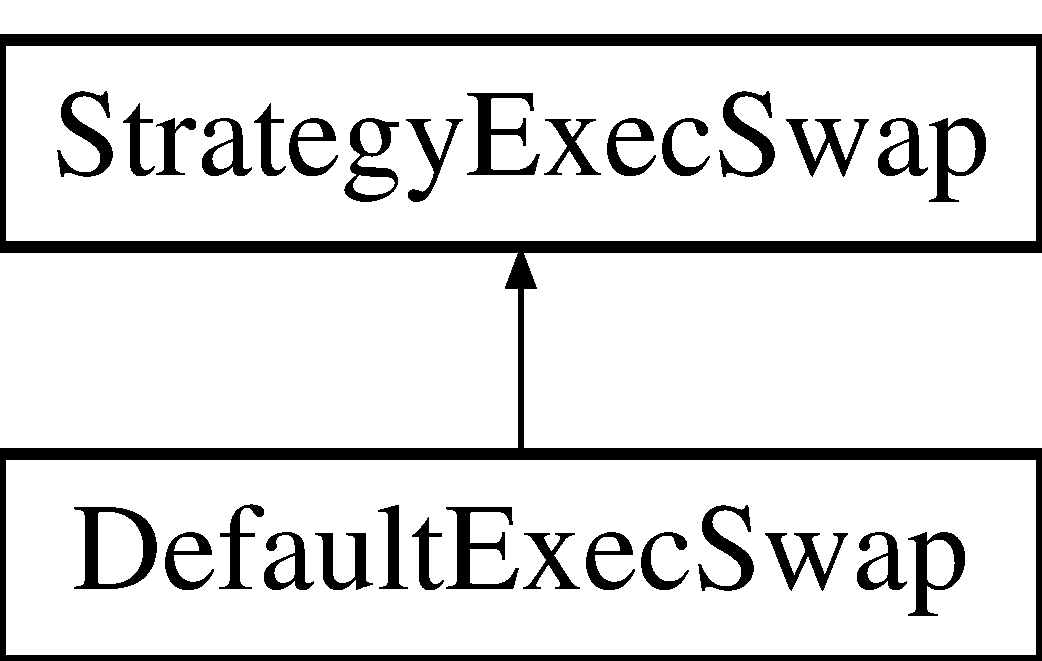
\includegraphics[height=2.000000cm]{classDefaultExecSwap}
\end{center}
\end{figure}
\subsection*{\-Public \-Member \-Functions}
\begin{DoxyCompactItemize}
\item 
void \hyperlink{classDefaultExecSwap_a97353521524f73e025572e1cab5b6b14}{executed\-Swap} (int k1, int k2)
\begin{DoxyCompactList}\small\item\em \-Wrapper when user function executed\-Swap is not defined. \end{DoxyCompactList}\end{DoxyCompactItemize}


\subsection{\-Detailed \-Description}
\-Default strategy to execute a swap. 

\subsection{\-Member \-Function \-Documentation}
\hypertarget{classDefaultExecSwap_a97353521524f73e025572e1cab5b6b14}{\index{\-Default\-Exec\-Swap@{\-Default\-Exec\-Swap}!executed\-Swap@{executed\-Swap}}
\index{executed\-Swap@{executed\-Swap}!DefaultExecSwap@{\-Default\-Exec\-Swap}}
\subsubsection[{executed\-Swap}]{\setlength{\rightskip}{0pt plus 5cm}void {\bf \-Default\-Exec\-Swap\-::executed\-Swap} (
\begin{DoxyParamCaption}
\item[{int}]{k1, }
\item[{int}]{k2}
\end{DoxyParamCaption}
)\hspace{0.3cm}{\ttfamily  \mbox{[}virtual\mbox{]}}}}\label{classDefaultExecSwap_a97353521524f73e025572e1cab5b6b14}


\-Wrapper when user function executed\-Swap is not defined. 


\begin{DoxyParams}{\-Parameters}
{\em k1} & and k2\-: variables to swap. \\
\hline
\end{DoxyParams}


\-Implements \hyperlink{classStrategyExecSwap_af233f7c89ae323aa30eb1c37c7dbe83c}{\-Strategy\-Exec\-Swap}.



\-The documentation for this class was generated from the following files\-:\begin{DoxyCompactItemize}
\item 
include/\hyperlink{default__exec__swap_8hpp}{default\-\_\-exec\-\_\-swap.\-hpp}\item 
src/\hyperlink{default__exec__swap_8cpp}{default\-\_\-exec\-\_\-swap.\-cpp}\end{DoxyCompactItemize}

\hypertarget{classDefaultNextI}{\section{\-Default\-Next\-I \-Class \-Reference}
\label{classDefaultNextI}\index{\-Default\-Next\-I@{\-Default\-Next\-I}}
}


\-Default strategy to return the next i (variable) to consider.  




{\ttfamily \#include $<$default\-\_\-next\-\_\-i.\-hpp$>$}

\-Inheritance diagram for \-Default\-Next\-I\-:\begin{figure}[H]
\begin{center}
\leavevmode
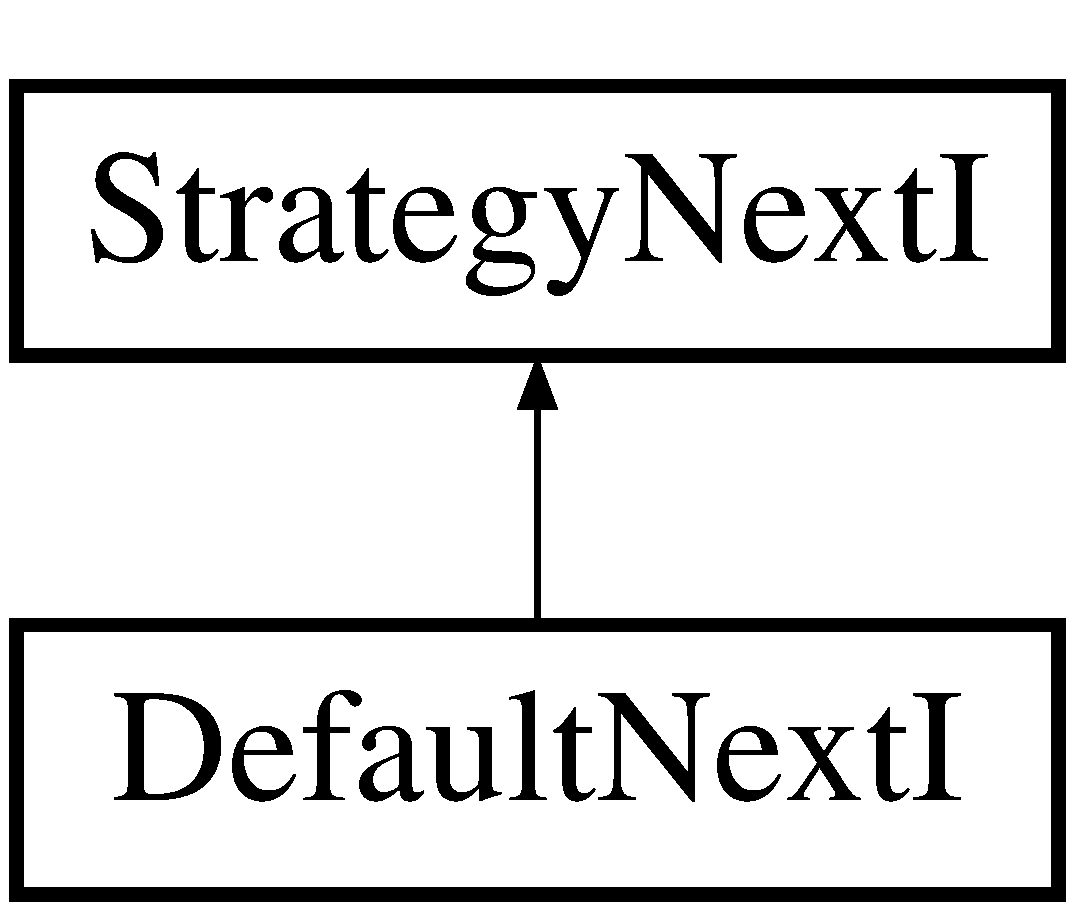
\includegraphics[height=2.000000cm]{classDefaultNextI}
\end{center}
\end{figure}
\subsection*{\-Public \-Member \-Functions}
\begin{DoxyCompactItemize}
\item 
int \hyperlink{classDefaultNextI_aa44893d3fa6e8b167774ff85d798ec3b}{next\-I} (int i)
\begin{DoxyCompactList}\small\item\em \-Wrapper when user function next\-I is not defined. \end{DoxyCompactList}\end{DoxyCompactItemize}


\subsection{\-Detailed \-Description}
\-Default strategy to return the next i (variable) to consider. 

\subsection{\-Member \-Function \-Documentation}
\hypertarget{classDefaultNextI_aa44893d3fa6e8b167774ff85d798ec3b}{\index{\-Default\-Next\-I@{\-Default\-Next\-I}!next\-I@{next\-I}}
\index{next\-I@{next\-I}!DefaultNextI@{\-Default\-Next\-I}}
\subsubsection[{next\-I}]{\setlength{\rightskip}{0pt plus 5cm}int {\bf \-Default\-Next\-I\-::next\-I} (
\begin{DoxyParamCaption}
\item[{int}]{i}
\end{DoxyParamCaption}
)\hspace{0.3cm}{\ttfamily  \mbox{[}virtual\mbox{]}}}}\label{classDefaultNextI_aa44893d3fa6e8b167774ff85d798ec3b}


\-Wrapper when user function next\-I is not defined. 


\begin{DoxyParams}{\-Parameters}
{\em i,\-:} & a variable. \\
\hline
\end{DoxyParams}
\begin{DoxyReturn}{\-Returns}
\-The next variable (i+1) 
\end{DoxyReturn}


\-Implements \hyperlink{classStrategyNextI_a3ae2498d9c8c316b9248e08c9d5ec3a3}{\-Strategy\-Next\-I}.



\-The documentation for this class was generated from the following file\-:\begin{DoxyCompactItemize}
\item 
include/\hyperlink{default__next__i_8hpp}{default\-\_\-next\-\_\-i.\-hpp}\end{DoxyCompactItemize}

\hypertarget{classDefaultNextJ}{\section{\-Default\-Next\-J \-Class \-Reference}
\label{classDefaultNextJ}\index{\-Default\-Next\-J@{\-Default\-Next\-J}}
}


\-Default strategy to return the next j (value) to consider, given i (variable)  




{\ttfamily \#include $<$default\-\_\-next\-\_\-j.\-h$>$}

\-Inheritance diagram for \-Default\-Next\-J\-:\begin{figure}[H]
\begin{center}
\leavevmode
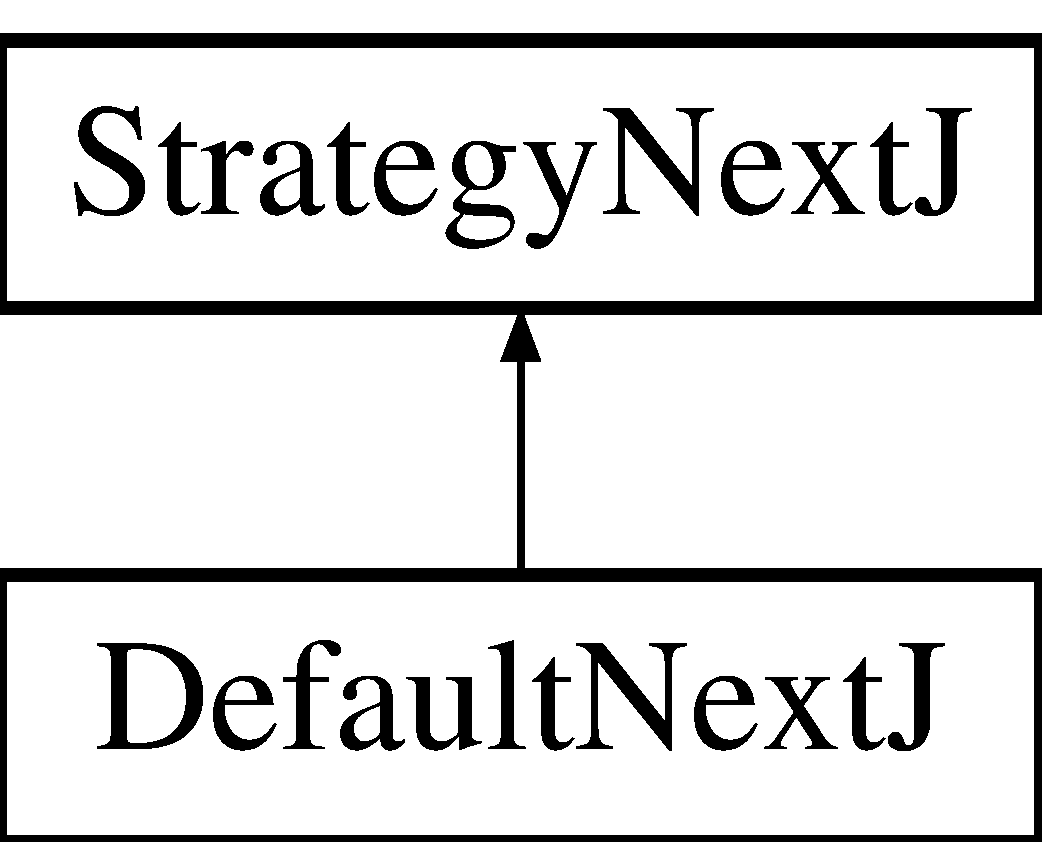
\includegraphics[height=2.000000cm]{classDefaultNextJ}
\end{center}
\end{figure}
\subsection*{\-Public \-Member \-Functions}
\begin{DoxyCompactItemize}
\item 
int \hyperlink{classDefaultNextJ_af3449e182609f056189cc1a22af0dd67}{next\-J} (int i, int j)
\begin{DoxyCompactList}\small\item\em \-Wrapper when user function next\-J is not defined. \end{DoxyCompactList}\end{DoxyCompactItemize}


\subsection{\-Detailed \-Description}
\-Default strategy to return the next j (value) to consider, given i (variable) 

\subsection{\-Member \-Function \-Documentation}
\hypertarget{classDefaultNextJ_af3449e182609f056189cc1a22af0dd67}{\index{\-Default\-Next\-J@{\-Default\-Next\-J}!next\-J@{next\-J}}
\index{next\-J@{next\-J}!DefaultNextJ@{\-Default\-Next\-J}}
\subsubsection[{next\-J}]{\setlength{\rightskip}{0pt plus 5cm}int {\bf \-Default\-Next\-J\-::next\-J} (
\begin{DoxyParamCaption}
\item[{int}]{i, }
\item[{int}]{j}
\end{DoxyParamCaption}
)\hspace{0.3cm}{\ttfamily  \mbox{[}inline, virtual\mbox{]}}}}\label{classDefaultNextJ_af3449e182609f056189cc1a22af0dd67}


\-Wrapper when user function next\-J is not defined. 


\begin{DoxyParams}{\-Parameters}
{\em i} & and j\-: two variables. \\
\hline
\end{DoxyParams}
\begin{DoxyReturn}{\-Returns}
\-The next j-\/variable (j+1), unless j $<$ 0 (then returns i+1) 
\end{DoxyReturn}


\-Implements \hyperlink{classStrategyNextJ_ab566c4e5827240b575d0e7445b7ba695}{\-Strategy\-Next\-J}.



\-The documentation for this class was generated from the following file\-:\begin{DoxyCompactItemize}
\item 
\hyperlink{default__next__j_8h}{default\-\_\-next\-\_\-j.\-h}\end{DoxyCompactItemize}

\hypertarget{classDefaultReset}{\section{\-Default\-Reset \-Class \-Reference}
\label{classDefaultReset}\index{\-Default\-Reset@{\-Default\-Reset}}
}


\-Default strategy to perform a reset.  




{\ttfamily \#include $<$default\-\_\-reset.\-hpp$>$}

\-Inheritance diagram for \-Default\-Reset\-:\begin{figure}[H]
\begin{center}
\leavevmode
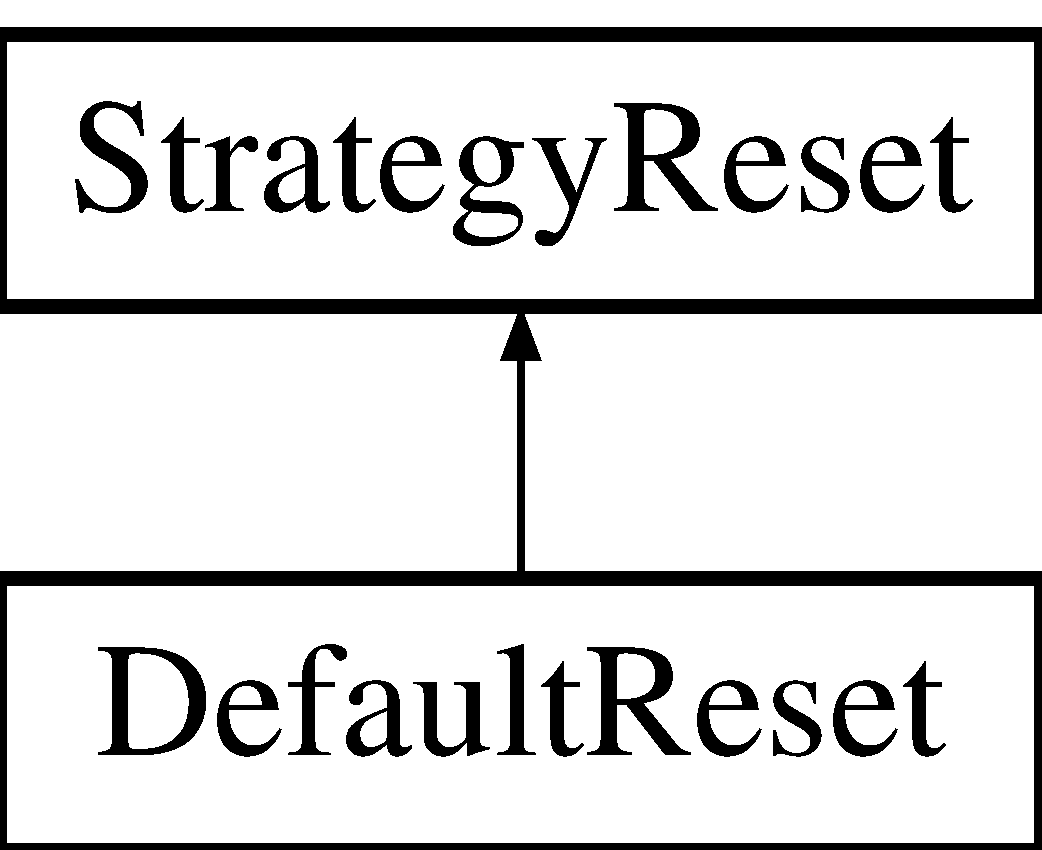
\includegraphics[height=2.000000cm]{classDefaultReset}
\end{center}
\end{figure}
\subsection*{\-Public \-Member \-Functions}
\begin{DoxyCompactItemize}
\item 
int \hyperlink{classDefaultReset_a82e58336172b51b8a8ce0369cbfd0a55}{reset} (int n, \hyperlink{classAdData}{\-Ad\-Data} $\ast$p\-\_\-ad)
\begin{DoxyCompactList}\small\item\em \-Wrapper when user function reset is not defined. \end{DoxyCompactList}\end{DoxyCompactItemize}


\subsection{\-Detailed \-Description}
\-Default strategy to perform a reset. 

\subsection{\-Member \-Function \-Documentation}
\hypertarget{classDefaultReset_a82e58336172b51b8a8ce0369cbfd0a55}{\index{\-Default\-Reset@{\-Default\-Reset}!reset@{reset}}
\index{reset@{reset}!DefaultReset@{\-Default\-Reset}}
\subsubsection[{reset}]{\setlength{\rightskip}{0pt plus 5cm}int {\bf \-Default\-Reset\-::reset} (
\begin{DoxyParamCaption}
\item[{int}]{n, }
\item[{{\bf \-Ad\-Data} $\ast$}]{p\-\_\-ad}
\end{DoxyParamCaption}
)\hspace{0.3cm}{\ttfamily  \mbox{[}virtual\mbox{]}}}}\label{classDefaultReset_a82e58336172b51b8a8ce0369cbfd0a55}


\-Wrapper when user function reset is not defined. 


\begin{DoxyParams}{\-Parameters}
{\em n,\-:} & number of reset loop to perform. p\-\_\-ad\-: pointer toward the configuration. \\
\hline
\end{DoxyParams}
\begin{DoxyReturn}{\-Returns}
\-The new cost, or -\/1 if unknown. 
\end{DoxyReturn}


\-Implements \hyperlink{classStrategyReset_af6cedf730c45825c61390455bd6f90a4}{\-Strategy\-Reset}.



\-The documentation for this class was generated from the following files\-:\begin{DoxyCompactItemize}
\item 
include/\hyperlink{default__reset_8hpp}{default\-\_\-reset.\-hpp}\item 
src/\hyperlink{default__reset_8cpp}{default\-\_\-reset.\-cpp}\end{DoxyCompactItemize}

\hypertarget{classMagicSquare}{
\section{MagicSquare Class Reference}
\label{classMagicSquare}\index{MagicSquare@{MagicSquare}}
}
\subsection*{Classes}
\begin{DoxyCompactItemize}
\item 
struct \hyperlink{structMagicSquare_1_1XRef}{XRef}
\end{DoxyCompactItemize}
\subsection*{Public Member Functions}
\begin{DoxyCompactItemize}
\item 
void \hyperlink{classMagicSquare_a3d43d7fa15f945e20491ec1125bd0d44}{Solve} (AdData $\ast$p\_\-ad)
\begin{DoxyCompactList}\small\item\em Initializations needed for the resolution. \item\end{DoxyCompactList}\item 
int \hyperlink{classMagicSquare_a7e45a2e9c128850bfb6717613a014fff}{Cost\_\-Of\_\-Solution} (int should\_\-be\_\-recorded)
\begin{DoxyCompactList}\small\item\em Computes the total cost of the current solution. Also computes errors on constraints for subsequent calls to Cost\_\-On\_\-Variable, Cost\_\-If\_\-Swap and Executed\_\-Swap. \item\end{DoxyCompactList}\item 
int \hyperlink{classMagicSquare_ae7ededec4689d278c83dc833c3a4b248}{Cost\_\-On\_\-Variable} (int k)
\begin{DoxyCompactList}\small\item\em Evaluates the error on a variable. \item\end{DoxyCompactList}\item 
int \hyperlink{classMagicSquare_a349868bc563431930a695795e8de84ed}{Cost\_\-If\_\-Swap} (int current\_\-cost, int k1, int k2)
\begin{DoxyCompactList}\small\item\em Computes the cost if we swap k1 and k2. No swaps are recorded. \item\end{DoxyCompactList}\item 
void \hyperlink{classMagicSquare_a4764e5e4485406f07f09c13307780757}{Executed\_\-Swap} (int k1, int k2)
\begin{DoxyCompactList}\small\item\em Records a swap between k1 and k2. \item\end{DoxyCompactList}\item 
void \hyperlink{classMagicSquare_a21aa228edea478e4240fb3c27024f670}{Init\_\-Parameters} (AdData $\ast$p\_\-ad)
\begin{DoxyCompactList}\small\item\em Initializes parameters like freeze\_\-swap, reset\_\-percent, ... \item\end{DoxyCompactList}\item 
int \hyperlink{classMagicSquare_a23b9fe6d1e267d66847e8bcb2b575738}{Check\_\-Solution} (AdData $\ast$p\_\-ad)
\begin{DoxyCompactList}\small\item\em Checks if the configuration is a solution. \item\end{DoxyCompactList}\end{DoxyCompactItemize}
\subsection*{Static Public Attributes}
\begin{DoxyCompactItemize}
\item 
\hypertarget{classMagicSquare_a526285b917194501dcf6656dc758926a}{
static int {\bfseries size}}
\label{classMagicSquare_a526285b917194501dcf6656dc758926a}

\item 
\hypertarget{classMagicSquare_a441c50e2d224b68c68b571ed6ca93506}{
static int $\ast$ {\bfseries sol}}
\label{classMagicSquare_a441c50e2d224b68c68b571ed6ca93506}

\item 
\hypertarget{classMagicSquare_a36cded7ec2d0e760cb344e413ff46218}{
static int {\bfseries square\_\-length}}
\label{classMagicSquare_a36cded7ec2d0e760cb344e413ff46218}

\item 
\hypertarget{classMagicSquare_a95a6a881885967a0c6b537eb91518729}{
static int {\bfseries square\_\-length\_\-m1}}
\label{classMagicSquare_a95a6a881885967a0c6b537eb91518729}

\item 
\hypertarget{classMagicSquare_acd21e15d520b34ba40e8f05b5cf6441d}{
static int {\bfseries square\_\-length\_\-p1}}
\label{classMagicSquare_acd21e15d520b34ba40e8f05b5cf6441d}

\item 
\hypertarget{classMagicSquare_a3b5958b6248adfca5b461fe1a39c038a}{
static int {\bfseries avg}}
\label{classMagicSquare_a3b5958b6248adfca5b461fe1a39c038a}

\item 
\hypertarget{classMagicSquare_aff35cc290ee4922a76489ab226c9d277}{
static int $\ast$ {\bfseries err\_\-l}}
\label{classMagicSquare_aff35cc290ee4922a76489ab226c9d277}

\item 
\hypertarget{classMagicSquare_ac849dbfa336a15280042b2fc2b372c79}{
static int $\ast$ {\bfseries err\_\-l\_\-abs}}
\label{classMagicSquare_ac849dbfa336a15280042b2fc2b372c79}

\item 
\hypertarget{classMagicSquare_ae3e52bf4e80df44fae1e301d6947ebd2}{
static int $\ast$ {\bfseries err\_\-c}}
\label{classMagicSquare_ae3e52bf4e80df44fae1e301d6947ebd2}

\item 
\hypertarget{classMagicSquare_a726c7a2306ae032767979c9fc66a07c0}{
static int $\ast$ {\bfseries err\_\-c\_\-abs}}
\label{classMagicSquare_a726c7a2306ae032767979c9fc66a07c0}

\item 
\hypertarget{classMagicSquare_ab91f3084c9031a0e81d722fc850920ef}{
static int {\bfseries err\_\-d1}}
\label{classMagicSquare_ab91f3084c9031a0e81d722fc850920ef}

\item 
\hypertarget{classMagicSquare_ab99a15ee17d12694f7e86f200f974709}{
static int {\bfseries err\_\-d1\_\-abs}}
\label{classMagicSquare_ab99a15ee17d12694f7e86f200f974709}

\item 
\hypertarget{classMagicSquare_a90978d9fed7ea4c793ed0daecdd711a3}{
static int {\bfseries err\_\-d2}}
\label{classMagicSquare_a90978d9fed7ea4c793ed0daecdd711a3}

\item 
\hypertarget{classMagicSquare_a0a229ebe88a15c6d9e3b8862be1b06ec}{
static int {\bfseries err\_\-d2\_\-abs}}
\label{classMagicSquare_a0a229ebe88a15c6d9e3b8862be1b06ec}

\item 
\hypertarget{classMagicSquare_a19af93510464733a26aeb3501716378d}{
static \hyperlink{structMagicSquare_1_1XRef}{XRef} $\ast$ {\bfseries xref}}
\label{classMagicSquare_a19af93510464733a26aeb3501716378d}

\end{DoxyCompactItemize}


\subsection{Member Function Documentation}
\hypertarget{classMagicSquare_a23b9fe6d1e267d66847e8bcb2b575738}{
\index{MagicSquare@{MagicSquare}!Check\_\-Solution@{Check\_\-Solution}}
\index{Check\_\-Solution@{Check\_\-Solution}!MagicSquare@{MagicSquare}}
\subsubsection[{Check\_\-Solution}]{\setlength{\rightskip}{0pt plus 5cm}int MagicSquare::Check\_\-Solution (
\begin{DoxyParamCaption}
\item[{AdData $\ast$}]{ p\_\-ad}
\end{DoxyParamCaption}
)}}
\label{classMagicSquare_a23b9fe6d1e267d66847e8bcb2b575738}


Checks if the configuration is a solution. 


\begin{DoxyParams}{Parameters}
\item[{\em p\_\-ad,:}]Pointer toward the current configuration. \end{DoxyParams}
\begin{DoxyReturn}{Returns}
1 if the configuration is a solution, 0 otherwise. 
\end{DoxyReturn}
\hypertarget{classMagicSquare_a349868bc563431930a695795e8de84ed}{
\index{MagicSquare@{MagicSquare}!Cost\_\-If\_\-Swap@{Cost\_\-If\_\-Swap}}
\index{Cost\_\-If\_\-Swap@{Cost\_\-If\_\-Swap}!MagicSquare@{MagicSquare}}
\subsubsection[{Cost\_\-If\_\-Swap}]{\setlength{\rightskip}{0pt plus 5cm}int MagicSquare::Cost\_\-If\_\-Swap (
\begin{DoxyParamCaption}
\item[{int}]{ current\_\-cost, }
\item[{int}]{ i, }
\item[{int}]{ j}
\end{DoxyParamCaption}
)}}
\label{classMagicSquare_a349868bc563431930a695795e8de84ed}


Computes the cost if we swap k1 and k2. No swaps are recorded. 


\begin{DoxyParams}{Parameters}
\item[{\em current\_\-cost,:}]the current cost when this function is called. \item[{\em i}]and j, the variables with which we simulate a swap to compute the resulting cost. \end{DoxyParams}
\begin{DoxyReturn}{Returns}
The cost if we swap variables i and j. 
\end{DoxyReturn}
\hypertarget{classMagicSquare_a7e45a2e9c128850bfb6717613a014fff}{
\index{MagicSquare@{MagicSquare}!Cost\_\-Of\_\-Solution@{Cost\_\-Of\_\-Solution}}
\index{Cost\_\-Of\_\-Solution@{Cost\_\-Of\_\-Solution}!MagicSquare@{MagicSquare}}
\subsubsection[{Cost\_\-Of\_\-Solution}]{\setlength{\rightskip}{0pt plus 5cm}int MagicSquare::Cost\_\-Of\_\-Solution (
\begin{DoxyParamCaption}
\item[{int}]{ should\_\-be\_\-recorded}
\end{DoxyParamCaption}
)}}
\label{classMagicSquare_a7e45a2e9c128850bfb6717613a014fff}


Computes the total cost of the current solution. Also computes errors on constraints for subsequent calls to Cost\_\-On\_\-Variable, Cost\_\-If\_\-Swap and Executed\_\-Swap. 


\begin{DoxyParams}{Parameters}
\item[{\em should\_\-be\_\-recorded,:}]dummy input. \end{DoxyParams}
\begin{DoxyReturn}{Returns}
The cost of the current configuration. 
\end{DoxyReturn}
\hypertarget{classMagicSquare_ae7ededec4689d278c83dc833c3a4b248}{
\index{MagicSquare@{MagicSquare}!Cost\_\-On\_\-Variable@{Cost\_\-On\_\-Variable}}
\index{Cost\_\-On\_\-Variable@{Cost\_\-On\_\-Variable}!MagicSquare@{MagicSquare}}
\subsubsection[{Cost\_\-On\_\-Variable}]{\setlength{\rightskip}{0pt plus 5cm}int MagicSquare::Cost\_\-On\_\-Variable (
\begin{DoxyParamCaption}
\item[{int}]{ k}
\end{DoxyParamCaption}
)}}
\label{classMagicSquare_ae7ededec4689d278c83dc833c3a4b248}


Evaluates the error on a variable. 


\begin{DoxyParams}{Parameters}
\item[{\em k,:}]the variable on which we project the cost. \end{DoxyParams}
\begin{DoxyReturn}{Returns}
The cost projected on variable k. 
\end{DoxyReturn}
\hypertarget{classMagicSquare_a4764e5e4485406f07f09c13307780757}{
\index{MagicSquare@{MagicSquare}!Executed\_\-Swap@{Executed\_\-Swap}}
\index{Executed\_\-Swap@{Executed\_\-Swap}!MagicSquare@{MagicSquare}}
\subsubsection[{Executed\_\-Swap}]{\setlength{\rightskip}{0pt plus 5cm}void MagicSquare::Executed\_\-Swap (
\begin{DoxyParamCaption}
\item[{int}]{ k1, }
\item[{int}]{ k2}
\end{DoxyParamCaption}
)}}
\label{classMagicSquare_a4764e5e4485406f07f09c13307780757}


Records a swap between k1 and k2. 


\begin{DoxyParams}{Parameters}
\item[{\em k1}]and k2: variables to swap. \end{DoxyParams}
\hypertarget{classMagicSquare_a21aa228edea478e4240fb3c27024f670}{
\index{MagicSquare@{MagicSquare}!Init\_\-Parameters@{Init\_\-Parameters}}
\index{Init\_\-Parameters@{Init\_\-Parameters}!MagicSquare@{MagicSquare}}
\subsubsection[{Init\_\-Parameters}]{\setlength{\rightskip}{0pt plus 5cm}void MagicSquare::Init\_\-Parameters (
\begin{DoxyParamCaption}
\item[{AdData $\ast$}]{ p\_\-ad}
\end{DoxyParamCaption}
)}}
\label{classMagicSquare_a21aa228edea478e4240fb3c27024f670}


Initializes parameters like freeze\_\-swap, reset\_\-percent, ... 


\begin{DoxyParams}{Parameters}
\item[{\em p\_\-ad,:}]Pointer toward the current configuration. \end{DoxyParams}
\hypertarget{classMagicSquare_a3d43d7fa15f945e20491ec1125bd0d44}{
\index{MagicSquare@{MagicSquare}!Solve@{Solve}}
\index{Solve@{Solve}!MagicSquare@{MagicSquare}}
\subsubsection[{Solve}]{\setlength{\rightskip}{0pt plus 5cm}void MagicSquare::Solve (
\begin{DoxyParamCaption}
\item[{AdData $\ast$}]{ p\_\-ad}
\end{DoxyParamCaption}
)}}
\label{classMagicSquare_a3d43d7fa15f945e20491ec1125bd0d44}


Initializations needed for the resolution. 


\begin{DoxyParams}{Parameters}
\item[{\em p\_\-ad,:}]Pointer toward the current configuration. \end{DoxyParams}


The documentation for this class was generated from the following files:\begin{DoxyCompactItemize}
\item 
\hyperlink{magic__square_8h}{magic\_\-square.h}\item 
\hyperlink{magic__square_8cpp}{magic\_\-square.cpp}\end{DoxyCompactItemize}

\hypertarget{classStrategyCostSwap}{\section{\-Strategy\-Cost\-Swap \-Class \-Reference}
\label{classStrategyCostSwap}\index{\-Strategy\-Cost\-Swap@{\-Strategy\-Cost\-Swap}}
}


\-Strategy \-Pattern to compute the cost of a swap.  




{\ttfamily \#include $<$strategy\-\_\-cost\-\_\-swap.\-hpp$>$}

\-Inheritance diagram for \-Strategy\-Cost\-Swap\-:\begin{figure}[H]
\begin{center}
\leavevmode
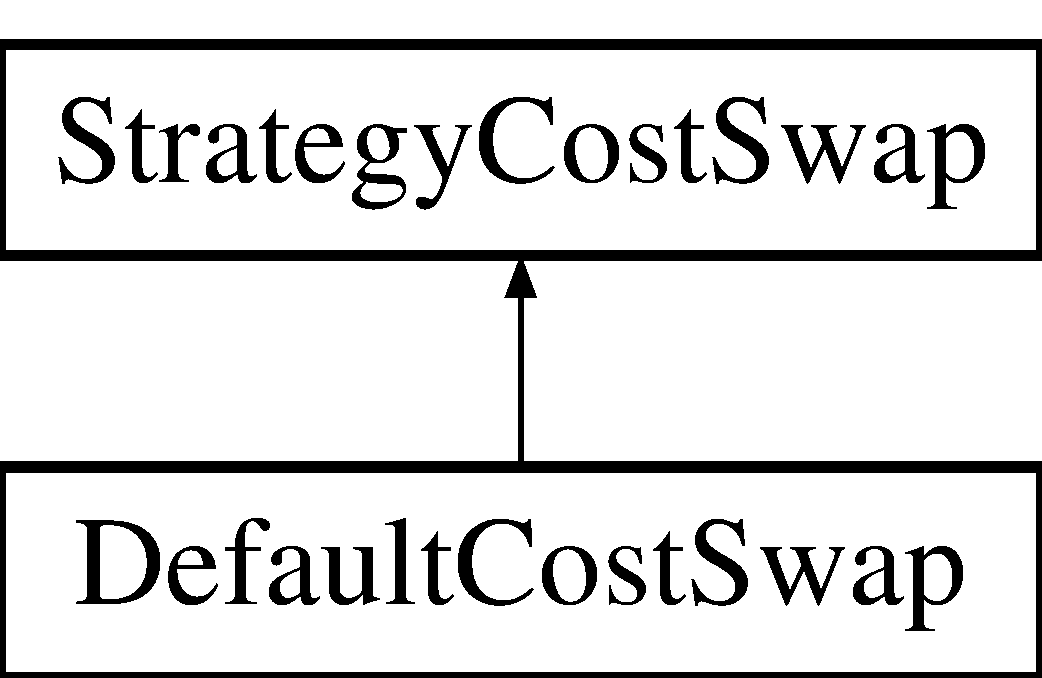
\includegraphics[height=2.000000cm]{classStrategyCostSwap}
\end{center}
\end{figure}
\subsection*{\-Public \-Member \-Functions}
\begin{DoxyCompactItemize}
\item 
virtual int \hyperlink{classStrategyCostSwap_a154e8db5c0e7cc22bd33942bbe4b8618}{cost\-If\-Swap} (int current\-Cost, int i, int j)=0
\begin{DoxyCompactList}\small\item\em \-Virtual wrapper when user function cost\-If\-Swap is not defined. \end{DoxyCompactList}\end{DoxyCompactItemize}


\subsection{\-Detailed \-Description}
\-Strategy \-Pattern to compute the cost of a swap. 

\subsection{\-Member \-Function \-Documentation}
\hypertarget{classStrategyCostSwap_a154e8db5c0e7cc22bd33942bbe4b8618}{\index{\-Strategy\-Cost\-Swap@{\-Strategy\-Cost\-Swap}!cost\-If\-Swap@{cost\-If\-Swap}}
\index{cost\-If\-Swap@{cost\-If\-Swap}!StrategyCostSwap@{\-Strategy\-Cost\-Swap}}
\subsubsection[{cost\-If\-Swap}]{\setlength{\rightskip}{0pt plus 5cm}int {\bf \-Strategy\-Cost\-Swap\-::cost\-If\-Swap} (
\begin{DoxyParamCaption}
\item[{int}]{current\-Cost, }
\item[{int}]{i, }
\item[{int}]{j}
\end{DoxyParamCaption}
)\hspace{0.3cm}{\ttfamily  \mbox{[}pure virtual\mbox{]}}}}\label{classStrategyCostSwap_a154e8db5c0e7cc22bd33942bbe4b8618}


\-Virtual wrapper when user function cost\-If\-Swap is not defined. 


\begin{DoxyParams}{\-Parameters}
{\em current\-Cost,\-:} & the current cost when this function is called. i and j, the variables with which we simulate a swap to compute the resulting cost. \\
\hline
\end{DoxyParams}
\begin{DoxyReturn}{\-Returns}
\-The cost if we swap variables i and j. 
\end{DoxyReturn}


\-Implemented in \hyperlink{classDefaultCostSwap_a62c43925fb3f931b12f92d3a1bbfc55f}{\-Default\-Cost\-Swap}.



\-The documentation for this class was generated from the following file\-:\begin{DoxyCompactItemize}
\item 
\hyperlink{strategy__cost__swap_8hpp}{strategy\-\_\-cost\-\_\-swap.\-hpp}\end{DoxyCompactItemize}

\hypertarget{classStrategyCostVar}{\section{\-Strategy\-Cost\-Var \-Class \-Reference}
\label{classStrategyCostVar}\index{\-Strategy\-Cost\-Var@{\-Strategy\-Cost\-Var}}
}


\-Strategy \-Pattern to compute the projected cost on a variable.  




{\ttfamily \#include $<$strategy\-\_\-cost\-\_\-var.\-hpp$>$}

\-Inheritance diagram for \-Strategy\-Cost\-Var\-:\begin{figure}[H]
\begin{center}
\leavevmode
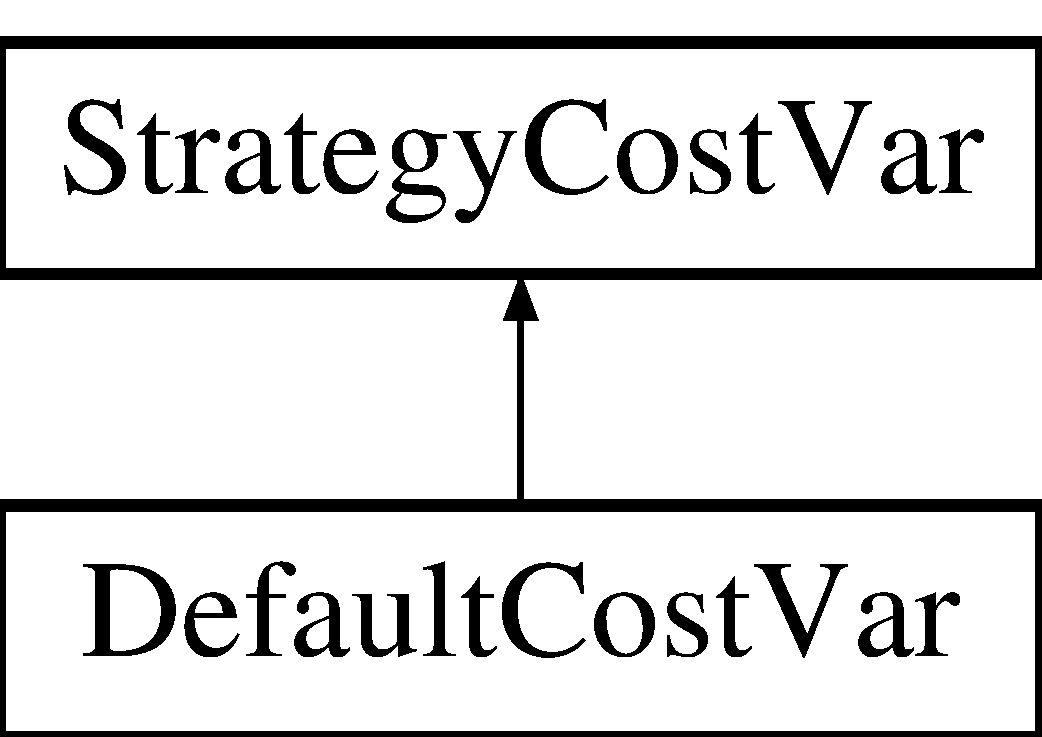
\includegraphics[height=2.000000cm]{classStrategyCostVar}
\end{center}
\end{figure}
\subsection*{\-Public \-Member \-Functions}
\begin{DoxyCompactItemize}
\item 
virtual int \hyperlink{classStrategyCostVar_a8381829dfa84b3460822aa0e3677a443}{cost\-On\-Variable} (int k)=0
\begin{DoxyCompactList}\small\item\em \-Wrapper when user function cost\-On\-Variable is not defined. \end{DoxyCompactList}\end{DoxyCompactItemize}


\subsection{\-Detailed \-Description}
\-Strategy \-Pattern to compute the projected cost on a variable. 

\subsection{\-Member \-Function \-Documentation}
\hypertarget{classStrategyCostVar_a8381829dfa84b3460822aa0e3677a443}{\index{\-Strategy\-Cost\-Var@{\-Strategy\-Cost\-Var}!cost\-On\-Variable@{cost\-On\-Variable}}
\index{cost\-On\-Variable@{cost\-On\-Variable}!StrategyCostVar@{\-Strategy\-Cost\-Var}}
\subsubsection[{cost\-On\-Variable}]{\setlength{\rightskip}{0pt plus 5cm}int {\bf \-Strategy\-Cost\-Var\-::cost\-On\-Variable} (
\begin{DoxyParamCaption}
\item[{int}]{k}
\end{DoxyParamCaption}
)\hspace{0.3cm}{\ttfamily  \mbox{[}pure virtual\mbox{]}}}}\label{classStrategyCostVar_a8381829dfa84b3460822aa0e3677a443}


\-Wrapper when user function cost\-On\-Variable is not defined. 


\begin{DoxyParams}{\-Parameters}
{\em k,\-:} & the variable on which we project the cost. \\
\hline
\end{DoxyParams}
\begin{DoxyReturn}{\-Returns}
\-The cost projected on variable k. 
\end{DoxyReturn}


\-Implemented in \hyperlink{classDefaultCostVar_a24820c1212f4e6f686156e9c0d3f2795}{\-Default\-Cost\-Var}.



\-The documentation for this class was generated from the following file\-:\begin{DoxyCompactItemize}
\item 
include/\hyperlink{strategy__cost__var_8hpp}{strategy\-\_\-cost\-\_\-var.\-hpp}\end{DoxyCompactItemize}

\hypertarget{classStrategyDisplaySol}{\section{\-Strategy\-Display\-Sol \-Class \-Reference}
\label{classStrategyDisplaySol}\index{\-Strategy\-Display\-Sol@{\-Strategy\-Display\-Sol}}
}


\-Strategy \-Pattern to display the solution.  




{\ttfamily \#include $<$strategy\-\_\-display\-\_\-sol.\-hpp$>$}

\-Inheritance diagram for \-Strategy\-Display\-Sol\-:\begin{figure}[H]
\begin{center}
\leavevmode
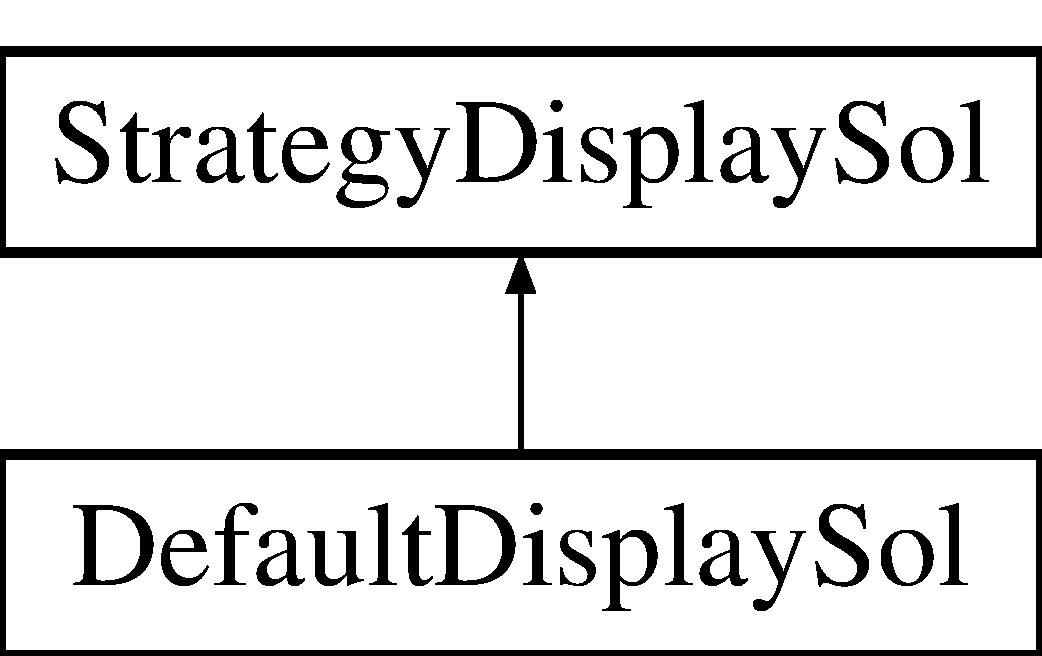
\includegraphics[height=2.000000cm]{classStrategyDisplaySol}
\end{center}
\end{figure}
\subsection*{\-Public \-Member \-Functions}
\begin{DoxyCompactItemize}
\item 
virtual void \hyperlink{classStrategyDisplaySol_aa4d70248e3281b868beb92875c8503c5}{display\-Solution} (\-Ad\-Data $\ast$p\-\_\-ad)=0
\begin{DoxyCompactList}\small\item\em \-Virtual wrapper when user function display\-Solution is not defined. \end{DoxyCompactList}\end{DoxyCompactItemize}


\subsection{\-Detailed \-Description}
\-Strategy \-Pattern to display the solution. 

\subsection{\-Member \-Function \-Documentation}
\hypertarget{classStrategyDisplaySol_aa4d70248e3281b868beb92875c8503c5}{\index{\-Strategy\-Display\-Sol@{\-Strategy\-Display\-Sol}!display\-Solution@{display\-Solution}}
\index{display\-Solution@{display\-Solution}!StrategyDisplaySol@{\-Strategy\-Display\-Sol}}
\subsubsection[{display\-Solution}]{\setlength{\rightskip}{0pt plus 5cm}void {\bf \-Strategy\-Display\-Sol\-::display\-Solution} (
\begin{DoxyParamCaption}
\item[{\-Ad\-Data $\ast$}]{p\-\_\-ad}
\end{DoxyParamCaption}
)\hspace{0.3cm}{\ttfamily  \mbox{[}pure virtual\mbox{]}}}}\label{classStrategyDisplaySol_aa4d70248e3281b868beb92875c8503c5}


\-Virtual wrapper when user function display\-Solution is not defined. 


\begin{DoxyParams}{\-Parameters}
{\em p\-\_\-ad,\-:} & \-Pointer toward the current configuration (or solution). \\
\hline
\end{DoxyParams}


\-Implemented in \hyperlink{classDefaultDisplaySol_ab80dde5db4b38e88dba892c5cf94c777}{\-Default\-Display\-Sol}.



\-The documentation for this class was generated from the following file\-:\begin{DoxyCompactItemize}
\item 
\hyperlink{strategy__display__sol_8hpp}{strategy\-\_\-display\-\_\-sol.\-hpp}\end{DoxyCompactItemize}

\hypertarget{classStrategyExecSwap}{\section{\-Strategy\-Exec\-Swap \-Class \-Reference}
\label{classStrategyExecSwap}\index{\-Strategy\-Exec\-Swap@{\-Strategy\-Exec\-Swap}}
}


\-Strategy \-Pattern to execute a swap.  




{\ttfamily \#include $<$strategy\-\_\-exec\-\_\-swap.\-hpp$>$}

\-Inheritance diagram for \-Strategy\-Exec\-Swap\-:\begin{figure}[H]
\begin{center}
\leavevmode
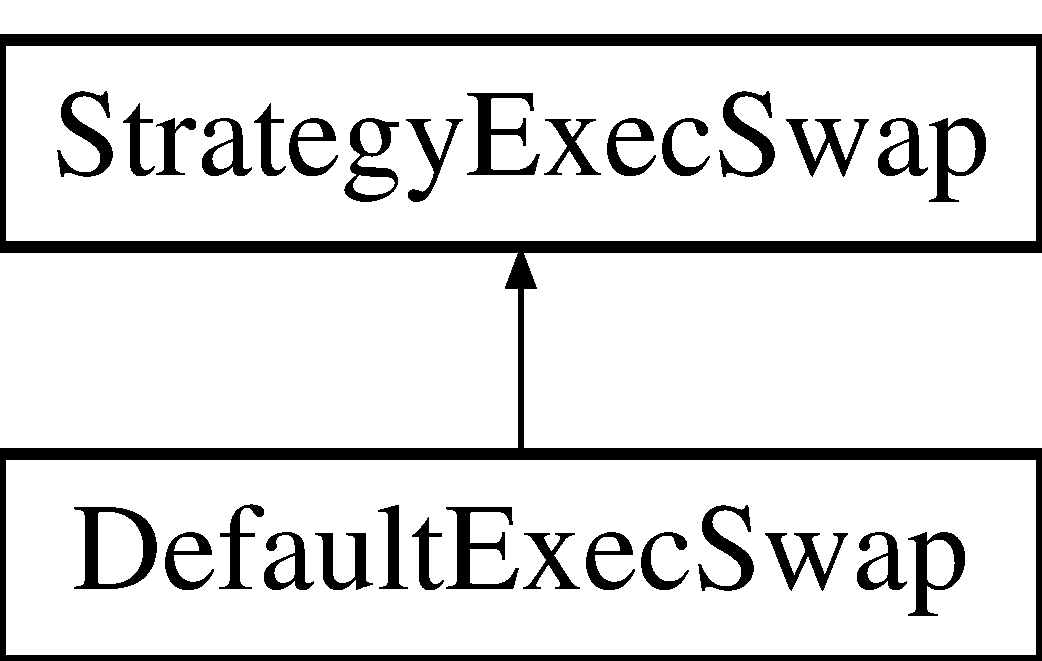
\includegraphics[height=2.000000cm]{classStrategyExecSwap}
\end{center}
\end{figure}
\subsection*{\-Public \-Member \-Functions}
\begin{DoxyCompactItemize}
\item 
virtual void \hyperlink{classStrategyExecSwap_af233f7c89ae323aa30eb1c37c7dbe83c}{executed\-Swap} (int k1, int k2)=0
\begin{DoxyCompactList}\small\item\em \-Virtual wrapper when user function executed\-Swap is not defined. \end{DoxyCompactList}\end{DoxyCompactItemize}


\subsection{\-Detailed \-Description}
\-Strategy \-Pattern to execute a swap. 

\subsection{\-Member \-Function \-Documentation}
\hypertarget{classStrategyExecSwap_af233f7c89ae323aa30eb1c37c7dbe83c}{\index{\-Strategy\-Exec\-Swap@{\-Strategy\-Exec\-Swap}!executed\-Swap@{executed\-Swap}}
\index{executed\-Swap@{executed\-Swap}!StrategyExecSwap@{\-Strategy\-Exec\-Swap}}
\subsubsection[{executed\-Swap}]{\setlength{\rightskip}{0pt plus 5cm}void {\bf \-Strategy\-Exec\-Swap\-::executed\-Swap} (
\begin{DoxyParamCaption}
\item[{int}]{k1, }
\item[{int}]{k2}
\end{DoxyParamCaption}
)\hspace{0.3cm}{\ttfamily  \mbox{[}pure virtual\mbox{]}}}}\label{classStrategyExecSwap_af233f7c89ae323aa30eb1c37c7dbe83c}


\-Virtual wrapper when user function executed\-Swap is not defined. 


\begin{DoxyParams}{\-Parameters}
{\em k1} & and k2\-: variables to swap. \\
\hline
\end{DoxyParams}


\-Implemented in \hyperlink{classDefaultExecSwap_a97353521524f73e025572e1cab5b6b14}{\-Default\-Exec\-Swap}.



\-The documentation for this class was generated from the following file\-:\begin{DoxyCompactItemize}
\item 
include/\hyperlink{strategy__exec__swap_8hpp}{strategy\-\_\-exec\-\_\-swap.\-hpp}\end{DoxyCompactItemize}

\hypertarget{classStrategyNextI}{\section{\-Strategy\-Next\-I \-Class \-Reference}
\label{classStrategyNextI}\index{\-Strategy\-Next\-I@{\-Strategy\-Next\-I}}
}


\-Strategy \-Pattern to return the next i (variable) to consider.  




{\ttfamily \#include $<$strategy\-\_\-next\-\_\-i.\-hpp$>$}

\-Inheritance diagram for \-Strategy\-Next\-I\-:\begin{figure}[H]
\begin{center}
\leavevmode
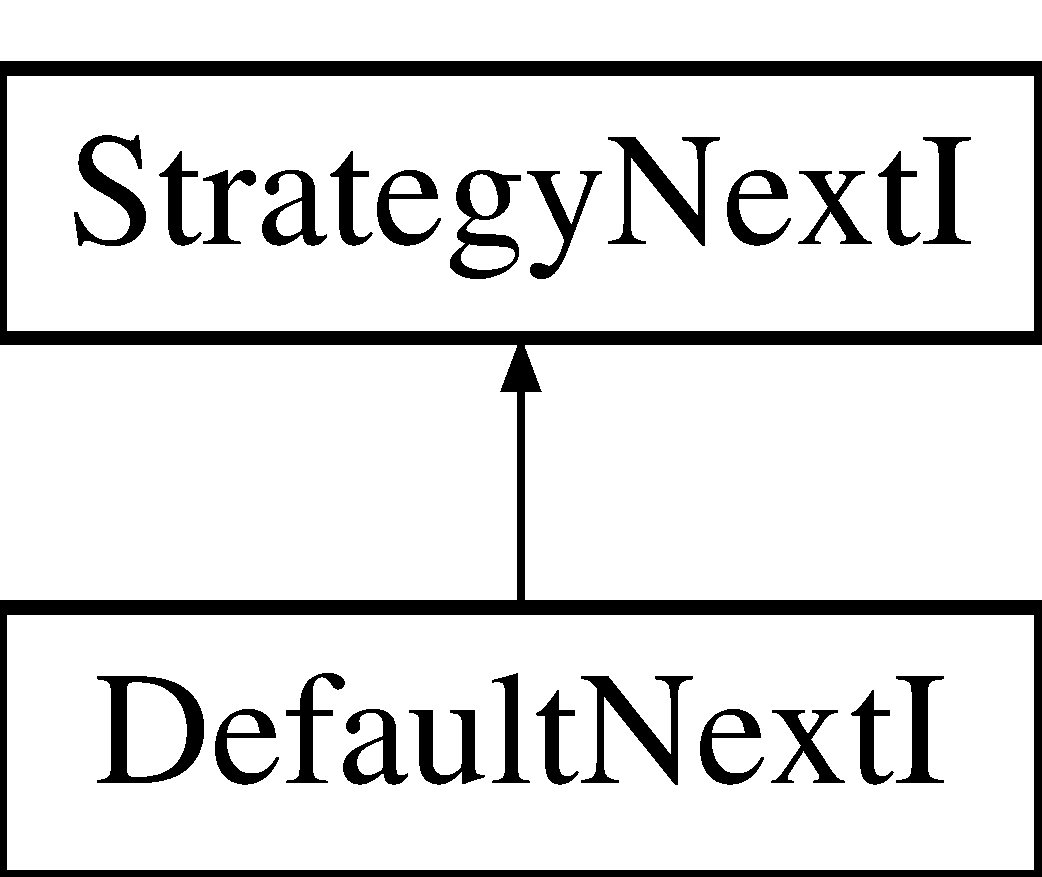
\includegraphics[height=2.000000cm]{classStrategyNextI}
\end{center}
\end{figure}
\subsection*{\-Public \-Member \-Functions}
\begin{DoxyCompactItemize}
\item 
virtual int \hyperlink{classStrategyNextI_a3ae2498d9c8c316b9248e08c9d5ec3a3}{next\-I} (int i)=0
\begin{DoxyCompactList}\small\item\em \-Virtual wrapper when user function next\-I is not defined. \end{DoxyCompactList}\end{DoxyCompactItemize}


\subsection{\-Detailed \-Description}
\-Strategy \-Pattern to return the next i (variable) to consider. 

\subsection{\-Member \-Function \-Documentation}
\hypertarget{classStrategyNextI_a3ae2498d9c8c316b9248e08c9d5ec3a3}{\index{\-Strategy\-Next\-I@{\-Strategy\-Next\-I}!next\-I@{next\-I}}
\index{next\-I@{next\-I}!StrategyNextI@{\-Strategy\-Next\-I}}
\subsubsection[{next\-I}]{\setlength{\rightskip}{0pt plus 5cm}int {\bf \-Strategy\-Next\-I\-::next\-I} (
\begin{DoxyParamCaption}
\item[{int}]{i}
\end{DoxyParamCaption}
)\hspace{0.3cm}{\ttfamily  \mbox{[}pure virtual\mbox{]}}}}\label{classStrategyNextI_a3ae2498d9c8c316b9248e08c9d5ec3a3}


\-Virtual wrapper when user function next\-I is not defined. 


\begin{DoxyParams}{\-Parameters}
{\em i,\-:} & a variable. \\
\hline
\end{DoxyParams}
\begin{DoxyReturn}{\-Returns}
\-The next variable (i+1) 
\end{DoxyReturn}


\-Implemented in \hyperlink{classDefaultNextI_aa44893d3fa6e8b167774ff85d798ec3b}{\-Default\-Next\-I}.



\-The documentation for this class was generated from the following file\-:\begin{DoxyCompactItemize}
\item 
\hyperlink{strategy__next__i_8hpp}{strategy\-\_\-next\-\_\-i.\-hpp}\end{DoxyCompactItemize}

\hypertarget{classStrategyNextJ}{\section{\-Strategy\-Next\-J \-Class \-Reference}
\label{classStrategyNextJ}\index{\-Strategy\-Next\-J@{\-Strategy\-Next\-J}}
}


\-Strategy \-Pattern to return the next j (value) to consider, given i (variable)  




{\ttfamily \#include $<$strategy\-\_\-next\-\_\-j.\-h$>$}

\-Inheritance diagram for \-Strategy\-Next\-J\-:\begin{figure}[H]
\begin{center}
\leavevmode
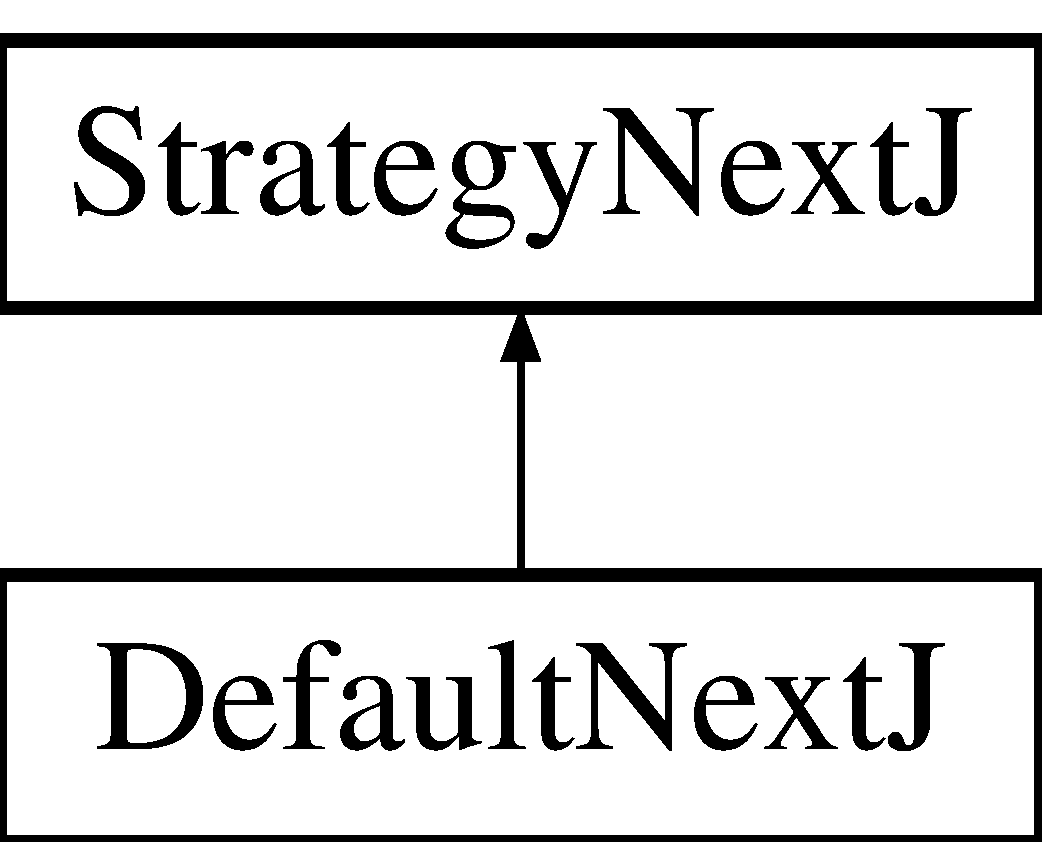
\includegraphics[height=2.000000cm]{classStrategyNextJ}
\end{center}
\end{figure}
\subsection*{\-Public \-Member \-Functions}
\begin{DoxyCompactItemize}
\item 
virtual int \hyperlink{classStrategyNextJ_ab566c4e5827240b575d0e7445b7ba695}{next\-J} (int i, int j)=0
\begin{DoxyCompactList}\small\item\em \-Virtual wrapper when user function next\-J is not defined. \end{DoxyCompactList}\end{DoxyCompactItemize}


\subsection{\-Detailed \-Description}
\-Strategy \-Pattern to return the next j (value) to consider, given i (variable) 

\subsection{\-Member \-Function \-Documentation}
\hypertarget{classStrategyNextJ_ab566c4e5827240b575d0e7445b7ba695}{\index{\-Strategy\-Next\-J@{\-Strategy\-Next\-J}!next\-J@{next\-J}}
\index{next\-J@{next\-J}!StrategyNextJ@{\-Strategy\-Next\-J}}
\subsubsection[{next\-J}]{\setlength{\rightskip}{0pt plus 5cm}int {\bf \-Strategy\-Next\-J\-::next\-J} (
\begin{DoxyParamCaption}
\item[{int}]{i, }
\item[{int}]{j}
\end{DoxyParamCaption}
)\hspace{0.3cm}{\ttfamily  \mbox{[}pure virtual\mbox{]}}}}\label{classStrategyNextJ_ab566c4e5827240b575d0e7445b7ba695}


\-Virtual wrapper when user function next\-J is not defined. 


\begin{DoxyParams}{\-Parameters}
{\em i} & and j\-: two variables. \\
\hline
\end{DoxyParams}
\begin{DoxyReturn}{\-Returns}
\-The next j-\/variable (j+1), unless j $<$ 0 (then returns i+1) 
\end{DoxyReturn}


\-Implemented in \hyperlink{classDefaultNextJ_af3449e182609f056189cc1a22af0dd67}{\-Default\-Next\-J}.



\-The documentation for this class was generated from the following file\-:\begin{DoxyCompactItemize}
\item 
\hyperlink{strategy__next__j_8h}{strategy\-\_\-next\-\_\-j.\-h}\end{DoxyCompactItemize}

\hypertarget{classStrategyReset}{\section{\-Strategy\-Reset \-Class \-Reference}
\label{classStrategyReset}\index{\-Strategy\-Reset@{\-Strategy\-Reset}}
}


\-Strategy \-Pattern to perform a reset.  




{\ttfamily \#include $<$strategy\-\_\-reset.\-hpp$>$}

\-Inheritance diagram for \-Strategy\-Reset\-:\begin{figure}[H]
\begin{center}
\leavevmode
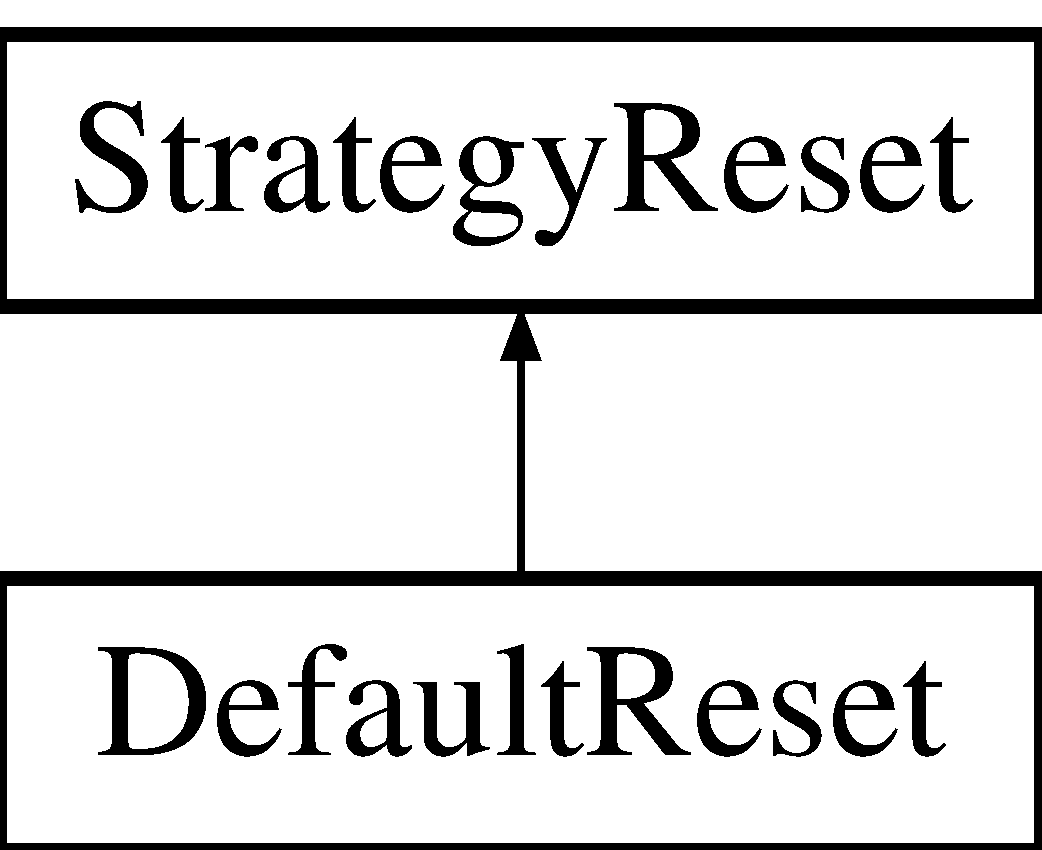
\includegraphics[height=2.000000cm]{classStrategyReset}
\end{center}
\end{figure}
\subsection*{\-Public \-Member \-Functions}
\begin{DoxyCompactItemize}
\item 
virtual int \hyperlink{classStrategyReset_af6cedf730c45825c61390455bd6f90a4}{reset} (int n, \hyperlink{classAdData}{\-Ad\-Data} $\ast$p\-\_\-ad)=0
\begin{DoxyCompactList}\small\item\em \-Virtual wrapper when user function reset is not defined. \end{DoxyCompactList}\end{DoxyCompactItemize}


\subsection{\-Detailed \-Description}
\-Strategy \-Pattern to perform a reset. 

\subsection{\-Member \-Function \-Documentation}
\hypertarget{classStrategyReset_af6cedf730c45825c61390455bd6f90a4}{\index{\-Strategy\-Reset@{\-Strategy\-Reset}!reset@{reset}}
\index{reset@{reset}!StrategyReset@{\-Strategy\-Reset}}
\subsubsection[{reset}]{\setlength{\rightskip}{0pt plus 5cm}int {\bf \-Strategy\-Reset\-::reset} (
\begin{DoxyParamCaption}
\item[{int}]{n, }
\item[{{\bf \-Ad\-Data} $\ast$}]{p\-\_\-ad}
\end{DoxyParamCaption}
)\hspace{0.3cm}{\ttfamily  \mbox{[}pure virtual\mbox{]}}}}\label{classStrategyReset_af6cedf730c45825c61390455bd6f90a4}


\-Virtual wrapper when user function reset is not defined. 


\begin{DoxyParams}{\-Parameters}
{\em n,\-:} & number of reset loop to perform. p\-\_\-ad\-: pointer toward the configuration. \\
\hline
\end{DoxyParams}
\begin{DoxyReturn}{\-Returns}
\-The new cost, or -\/1 if unknown. 
\end{DoxyReturn}


\-Implemented in \hyperlink{classDefaultReset_a82e58336172b51b8a8ce0369cbfd0a55}{\-Default\-Reset}.



\-The documentation for this class was generated from the following file\-:\begin{DoxyCompactItemize}
\item 
include/\hyperlink{strategy__reset_8hpp}{strategy\-\_\-reset.\-hpp}\end{DoxyCompactItemize}

\hypertarget{structMagicSquare_1_1XRef}{\section{\-Magic\-Square\-:\-:\-X\-Ref \-Struct \-Reference}
\label{structMagicSquare_1_1XRef}\index{\-Magic\-Square\-::\-X\-Ref@{\-Magic\-Square\-::\-X\-Ref}}
}
\subsection*{\-Public \-Attributes}
\begin{DoxyCompactItemize}
\item 
\hypertarget{structMagicSquare_1_1XRef_a9da1ebfcf74bd506f8705783e92d764f}{unsigned int {\bfseries d1}\-:1}\label{structMagicSquare_1_1XRef_a9da1ebfcf74bd506f8705783e92d764f}

\item 
\hypertarget{structMagicSquare_1_1XRef_ad1d07d5c5ff273961e4329af5a8ff2d0}{unsigned int {\bfseries d2}\-:1}\label{structMagicSquare_1_1XRef_ad1d07d5c5ff273961e4329af5a8ff2d0}

\item 
\hypertarget{structMagicSquare_1_1XRef_af86bd806c544303f25ee0feca31afc57}{unsigned int {\bfseries l}\-:15}\label{structMagicSquare_1_1XRef_af86bd806c544303f25ee0feca31afc57}

\item 
\hypertarget{structMagicSquare_1_1XRef_aac7b71199e3718a13b6a7853469ace7e}{unsigned int {\bfseries c}\-:15}\label{structMagicSquare_1_1XRef_aac7b71199e3718a13b6a7853469ace7e}

\end{DoxyCompactItemize}


\-The documentation for this struct was generated from the following file\-:\begin{DoxyCompactItemize}
\item 
\hyperlink{magic__square_8h}{magic\-\_\-square.\-h}\end{DoxyCompactItemize}

\chapter{\-File \-Documentation}
\hypertarget{bench_8cpp}{
\section{bench.cpp File Reference}
\label{bench_8cpp}\index{bench.cpp@{bench.cpp}}
}


benchmark mother class  


{\ttfamily \#include \char`\"{}bench.h\char`\"{}}\par


\subsection{Detailed Description}
benchmark mother class Adaptive search C++

\begin{DoxyAuthor}{Author}
Florian Richoux 
\end{DoxyAuthor}
\begin{DoxyDate}{Date}
2011-\/09-\/03
\end{DoxyDate}
Copyright (C) 2011 JFLI 
\hypertarget{bench_8hpp}{\section{include/bench.hpp \-File \-Reference}
\label{bench_8hpp}\index{include/bench.\-hpp@{include/bench.\-hpp}}
}


\-Benchmark mother class.  


\subsection*{\-Classes}
\begin{DoxyCompactItemize}
\item 
class \hyperlink{classBench}{\-Bench}
\begin{DoxyCompactList}\small\item\em \-Benchmark mother class. \end{DoxyCompactList}\end{DoxyCompactItemize}


\subsection{\-Detailed \-Description}
\-Benchmark mother class. \-Adaptive \-Framework

\begin{DoxyAuthor}{\-Author}
\-Florian \-Richoux 
\end{DoxyAuthor}
\begin{DoxyDate}{\-Date}
2013-\/01-\/21 
\end{DoxyDate}

\hypertarget{default__cost__swap_8cpp}{\section{default\-\_\-cost\-\_\-swap.\-cpp \-File \-Reference}
\label{default__cost__swap_8cpp}\index{default\-\_\-cost\-\_\-swap.\-cpp@{default\-\_\-cost\-\_\-swap.\-cpp}}
}


\-Default strategy to compute the cost of a swap.  




\subsection{\-Detailed \-Description}
\-Default strategy to compute the cost of a swap. \-Adaptive search \-C++

\begin{DoxyAuthor}{\-Author}
\-Florian \-Richoux 
\end{DoxyAuthor}
\begin{DoxyDate}{\-Date}
2013-\/01-\/21 
\end{DoxyDate}

\hypertarget{default__cost__swap_8hpp}{\section{include/default\-\_\-cost\-\_\-swap.hpp \-File \-Reference}
\label{default__cost__swap_8hpp}\index{include/default\-\_\-cost\-\_\-swap.\-hpp@{include/default\-\_\-cost\-\_\-swap.\-hpp}}
}


\-Default strategy to compute the cost of a swap.  


\subsection*{\-Classes}
\begin{DoxyCompactItemize}
\item 
class \hyperlink{classDefaultCostSwap}{\-Default\-Cost\-Swap}
\begin{DoxyCompactList}\small\item\em \-Default strategy to compute the cost of a swap. \end{DoxyCompactList}\end{DoxyCompactItemize}


\subsection{\-Detailed \-Description}
\-Default strategy to compute the cost of a swap. \-Adaptive search \-C++

\begin{DoxyAuthor}{\-Author}
\-Florian \-Richoux 
\end{DoxyAuthor}
\begin{DoxyDate}{\-Date}
2013-\/01-\/21 
\end{DoxyDate}

\hypertarget{default__cost__var_8cpp}{\section{src/default\-\_\-cost\-\_\-var.cpp \-File \-Reference}
\label{default__cost__var_8cpp}\index{src/default\-\_\-cost\-\_\-var.\-cpp@{src/default\-\_\-cost\-\_\-var.\-cpp}}
}


\-Default strategy to compute the projected cost on a variable.  




\subsection{\-Detailed \-Description}
\-Default strategy to compute the projected cost on a variable. \-Adaptive \-Framework

\begin{DoxyAuthor}{\-Author}
\-Florian \-Richoux 
\end{DoxyAuthor}
\begin{DoxyDate}{\-Date}
2013-\/01-\/21 
\end{DoxyDate}

\hypertarget{default__cost__var_8hpp}{\section{include/default\-\_\-cost\-\_\-var.hpp \-File \-Reference}
\label{default__cost__var_8hpp}\index{include/default\-\_\-cost\-\_\-var.\-hpp@{include/default\-\_\-cost\-\_\-var.\-hpp}}
}


\-Default strategy to compute the projected cost on a variable.  


\subsection*{\-Classes}
\begin{DoxyCompactItemize}
\item 
class \hyperlink{classDefaultCostVar}{\-Default\-Cost\-Var}
\begin{DoxyCompactList}\small\item\em \-Default strategy to compute the cost of a swap. \end{DoxyCompactList}\end{DoxyCompactItemize}


\subsection{\-Detailed \-Description}
\-Default strategy to compute the projected cost on a variable. \-Adaptive \-Framework

\begin{DoxyAuthor}{\-Author}
\-Florian \-Richoux 
\end{DoxyAuthor}
\begin{DoxyDate}{\-Date}
2013-\/01-\/21 
\end{DoxyDate}

\hypertarget{default__display__sol_8cpp}{\section{src/default\-\_\-display\-\_\-sol.cpp \-File \-Reference}
\label{default__display__sol_8cpp}\index{src/default\-\_\-display\-\_\-sol.\-cpp@{src/default\-\_\-display\-\_\-sol.\-cpp}}
}


\-Default strategy to display the solution.  




\subsection{\-Detailed \-Description}
\-Default strategy to display the solution. \-Adaptive \-Framework

\begin{DoxyAuthor}{\-Author}
\-Florian \-Richoux 
\end{DoxyAuthor}
\begin{DoxyDate}{\-Date}
2013-\/01-\/21 
\end{DoxyDate}

\hypertarget{default__display__sol_8hpp}{\section{default\-\_\-display\-\_\-sol.\-hpp \-File \-Reference}
\label{default__display__sol_8hpp}\index{default\-\_\-display\-\_\-sol.\-hpp@{default\-\_\-display\-\_\-sol.\-hpp}}
}


\-Default strategy to display the solution.  


\subsection*{\-Classes}
\begin{DoxyCompactItemize}
\item 
class \hyperlink{classDefaultDisplaySol}{\-Default\-Display\-Sol}
\begin{DoxyCompactList}\small\item\em \-Default strategy to display the solution. \end{DoxyCompactList}\end{DoxyCompactItemize}


\subsection{\-Detailed \-Description}
\-Default strategy to display the solution. \-Adaptive search \-C++

\begin{DoxyAuthor}{\-Author}
\-Florian \-Richoux 
\end{DoxyAuthor}
\begin{DoxyDate}{\-Date}
2013-\/01-\/21 
\end{DoxyDate}

\hypertarget{default__exec__swap_8cpp}{\section{src/default\-\_\-exec\-\_\-swap.cpp \-File \-Reference}
\label{default__exec__swap_8cpp}\index{src/default\-\_\-exec\-\_\-swap.\-cpp@{src/default\-\_\-exec\-\_\-swap.\-cpp}}
}


\-Default strategy to execute a swap.  




\subsection{\-Detailed \-Description}
\-Default strategy to execute a swap. \-Adaptive \-Framework

\begin{DoxyAuthor}{\-Author}
\-Florian \-Richoux 
\end{DoxyAuthor}
\begin{DoxyDate}{\-Date}
2013-\/01-\/21 
\end{DoxyDate}

\hypertarget{default__exec__swap_8hpp}{\section{include/default\-\_\-exec\-\_\-swap.hpp \-File \-Reference}
\label{default__exec__swap_8hpp}\index{include/default\-\_\-exec\-\_\-swap.\-hpp@{include/default\-\_\-exec\-\_\-swap.\-hpp}}
}


\-Default strategy to execute a swap.  


\subsection*{\-Classes}
\begin{DoxyCompactItemize}
\item 
class \hyperlink{classDefaultExecSwap}{\-Default\-Exec\-Swap}
\begin{DoxyCompactList}\small\item\em \-Default strategy to execute a swap. \end{DoxyCompactList}\end{DoxyCompactItemize}


\subsection{\-Detailed \-Description}
\-Default strategy to execute a swap. \-Adaptive search \-C++

\begin{DoxyAuthor}{\-Author}
\-Florian \-Richoux 
\end{DoxyAuthor}
\begin{DoxyDate}{\-Date}
2013-\/01-\/21 
\end{DoxyDate}

\hypertarget{default__next__i_8cpp}{\section{default\-\_\-next\-\_\-i.\-cpp \-File \-Reference}
\label{default__next__i_8cpp}\index{default\-\_\-next\-\_\-i.\-cpp@{default\-\_\-next\-\_\-i.\-cpp}}
}


\-Default strategy to return the next i (variable) to consider.  




\subsection{\-Detailed \-Description}
\-Default strategy to return the next i (variable) to consider. \-Adaptive search \-C++

\begin{DoxyAuthor}{\-Author}
\-Florian \-Richoux 
\end{DoxyAuthor}
\begin{DoxyDate}{\-Date}
2013-\/01-\/21 
\end{DoxyDate}

\hypertarget{default__next__i_8hpp}{\section{include/default\-\_\-next\-\_\-i.hpp \-File \-Reference}
\label{default__next__i_8hpp}\index{include/default\-\_\-next\-\_\-i.\-hpp@{include/default\-\_\-next\-\_\-i.\-hpp}}
}


\-Default strategy to return the next i (variable) to consider.  


\subsection*{\-Classes}
\begin{DoxyCompactItemize}
\item 
class \hyperlink{classDefaultNextI}{\-Default\-Next\-I}
\begin{DoxyCompactList}\small\item\em \-Default strategy to return the next i (variable) to consider. \end{DoxyCompactList}\end{DoxyCompactItemize}


\subsection{\-Detailed \-Description}
\-Default strategy to return the next i (variable) to consider. \-Adaptive \-Framework

\begin{DoxyAuthor}{\-Author}
\-Florian \-Richoux 
\end{DoxyAuthor}
\begin{DoxyDate}{\-Date}
2013-\/01-\/21 
\end{DoxyDate}

\hypertarget{default__next__j_8cpp}{\section{default\-\_\-next\-\_\-j.\-cpp \-File \-Reference}
\label{default__next__j_8cpp}\index{default\-\_\-next\-\_\-j.\-cpp@{default\-\_\-next\-\_\-j.\-cpp}}
}


\-Default strategy to return the next j (value) to consider, given i (variable)  




\subsection{\-Detailed \-Description}
\-Default strategy to return the next j (value) to consider, given i (variable) \-Adaptive search \-C++

\begin{DoxyAuthor}{\-Author}
\-Florian \-Richoux 
\end{DoxyAuthor}
\begin{DoxyDate}{\-Date}
2013-\/01-\/21 
\end{DoxyDate}

\hypertarget{default__next__j_8hpp}{\section{default\-\_\-next\-\_\-j.\-hpp \-File \-Reference}
\label{default__next__j_8hpp}\index{default\-\_\-next\-\_\-j.\-hpp@{default\-\_\-next\-\_\-j.\-hpp}}
}


\-Default strategy to return the next j (value) to consider, given i (variable)  


\subsection*{\-Classes}
\begin{DoxyCompactItemize}
\item 
class \hyperlink{classDefaultNextJ}{\-Default\-Next\-J}
\begin{DoxyCompactList}\small\item\em \-Default strategy to return the next j (value) to consider, given i (variable) \end{DoxyCompactList}\end{DoxyCompactItemize}


\subsection{\-Detailed \-Description}
\-Default strategy to return the next j (value) to consider, given i (variable) \-Adaptive search \-C++

\begin{DoxyAuthor}{\-Author}
\-Florian \-Richoux 
\end{DoxyAuthor}
\begin{DoxyDate}{\-Date}
2013-\/01-\/21 
\end{DoxyDate}

\hypertarget{default__reset_8cpp}{\section{src/default\-\_\-reset.cpp \-File \-Reference}
\label{default__reset_8cpp}\index{src/default\-\_\-reset.\-cpp@{src/default\-\_\-reset.\-cpp}}
}


\-Default strategy to perform a reset.  




\subsection{\-Detailed \-Description}
\-Default strategy to perform a reset. \-Adaptive search \-C++

\begin{DoxyAuthor}{\-Author}
\-Florian \-Richoux 
\end{DoxyAuthor}
\begin{DoxyDate}{\-Date}
2013-\/01-\/21 
\end{DoxyDate}

\hypertarget{default__reset_8hpp}{\section{include/default\-\_\-reset.hpp \-File \-Reference}
\label{default__reset_8hpp}\index{include/default\-\_\-reset.\-hpp@{include/default\-\_\-reset.\-hpp}}
}


\-Default strategy to perform a reset.  


\subsection*{\-Classes}
\begin{DoxyCompactItemize}
\item 
class \hyperlink{classDefaultReset}{\-Default\-Reset}
\begin{DoxyCompactList}\small\item\em \-Default strategy to perform a reset. \end{DoxyCompactList}\end{DoxyCompactItemize}


\subsection{\-Detailed \-Description}
\-Default strategy to perform a reset. \-Adaptive search \-C++

\begin{DoxyAuthor}{\-Author}
\-Florian \-Richoux 
\end{DoxyAuthor}
\begin{DoxyDate}{\-Date}
2013-\/01-\/21 
\end{DoxyDate}

\hypertarget{magic__square_8cpp}{\section{magic\-\_\-square.\-cpp \-File \-Reference}
\label{magic__square_8cpp}\index{magic\-\_\-square.\-cpp@{magic\-\_\-square.\-cpp}}
}


\-Magic \-Square benchmark.  


\subsection*{\-Defines}
\begin{DoxyCompactItemize}
\item 
\hypertarget{magic__square_8cpp_a9fd3fc702371e8304ba86701eb081e8e}{\#define {\bfseries \-Adjust\-L}(r, diff, k)~r = r -\/ err\-\_\-l\-\_\-abs\mbox{[}k\mbox{]} + abs(err\-\_\-l\mbox{[}k\mbox{]} + diff)}\label{magic__square_8cpp_a9fd3fc702371e8304ba86701eb081e8e}

\item 
\hypertarget{magic__square_8cpp_ae4a27848134efefc7ca1330e4cf87542}{\#define {\bfseries \-Adjust\-C}(r, diff, k)~r = r -\/ err\-\_\-c\-\_\-abs\mbox{[}k\mbox{]} + abs(err\-\_\-c\mbox{[}k\mbox{]} + diff)}\label{magic__square_8cpp_ae4a27848134efefc7ca1330e4cf87542}

\item 
\hypertarget{magic__square_8cpp_a9f6dd1b0dc79411bd2c43c6fbc971f57}{\#define {\bfseries \-Adjust\-D1}(r, diff)~r = r -\/ err\-\_\-d1\-\_\-abs   + abs(err\-\_\-d1   + diff)}\label{magic__square_8cpp_a9f6dd1b0dc79411bd2c43c6fbc971f57}

\item 
\hypertarget{magic__square_8cpp_a3d83b80a143bc2743324fa13522fef42}{\#define {\bfseries \-Adjust\-D2}(r, diff)~r = r -\/ err\-\_\-d2\-\_\-abs   + abs(err\-\_\-d2   + diff)}\label{magic__square_8cpp_a3d83b80a143bc2743324fa13522fef42}

\end{DoxyCompactItemize}
\subsection*{\-Variables}
\begin{DoxyCompactItemize}
\item 
\hypertarget{magic__square_8cpp_a9d5b699859472f64d01758fa31a98546}{int {\bfseries param\-\_\-needed} = 1}\label{magic__square_8cpp_a9d5b699859472f64d01758fa31a98546}

\end{DoxyCompactItemize}


\subsection{\-Detailed \-Description}
\-Magic \-Square benchmark. \-Adaptive search \-C++

\begin{DoxyAuthor}{\-Author}
\-Florian \-Richoux 
\end{DoxyAuthor}
\begin{DoxyDate}{\-Date}
2011-\/09-\/03
\end{DoxyDate}
\-Copyright (\-C) 2011 \-J\-F\-L\-I 
\hypertarget{magic__square_8hpp}{\section{magic\-\_\-square.\-hpp \-File \-Reference}
\label{magic__square_8hpp}\index{magic\-\_\-square.\-hpp@{magic\-\_\-square.\-hpp}}
}


\-Magic \-Square benchmark.  


\subsection*{\-Classes}
\begin{DoxyCompactItemize}
\item 
class \hyperlink{classMagicSquare}{\-Magic\-Square}
\begin{DoxyCompactList}\small\item\em \-Magic \-Square benchmark. \end{DoxyCompactList}\item 
struct \hyperlink{structMagicSquare_1_1XRef}{\-Magic\-Square\-::\-X\-Ref}
\end{DoxyCompactItemize}
\subsection*{\-Defines}
\begin{DoxyCompactItemize}
\item 
\hypertarget{magic__square_8hpp_a08fe385c0455a06d2d4713f87ea3b168}{\#define {\bfseries \-X\-Set}(xr, line, col, diag1, diag2)~xr.\-l = line; xr.\-c = col; xr.\-d1 = diag1; xr.\-d2 = diag2}\label{magic__square_8hpp_a08fe385c0455a06d2d4713f87ea3b168}

\item 
\hypertarget{magic__square_8hpp_abc9c2142ff5fbe9e0014f12484ad19c9}{\#define {\bfseries \-X\-Get\-L}(xr)~xr.\-l}\label{magic__square_8hpp_abc9c2142ff5fbe9e0014f12484ad19c9}

\item 
\hypertarget{magic__square_8hpp_aa54a553c860cec32c9c47b26044820fe}{\#define {\bfseries \-X\-Get\-C}(xr)~xr.\-c}\label{magic__square_8hpp_aa54a553c860cec32c9c47b26044820fe}

\item 
\hypertarget{magic__square_8hpp_aae4bd6187bbf650594614dc43135b1bf}{\#define {\bfseries \-X\-Is\-On\-D1}(xr)~(xr.\-d1 != 0)}\label{magic__square_8hpp_aae4bd6187bbf650594614dc43135b1bf}

\item 
\hypertarget{magic__square_8hpp_a8dc1853267f4288b2d9d0f1a6b356d2b}{\#define {\bfseries \-X\-Is\-On\-D2}(xr)~(xr.\-d2 != 0)}\label{magic__square_8hpp_a8dc1853267f4288b2d9d0f1a6b356d2b}

\end{DoxyCompactItemize}


\subsection{\-Detailed \-Description}
\-Magic \-Square benchmark. \-Adaptive search \-C++

\begin{DoxyAuthor}{\-Author}
\-Florian \-Richoux 
\end{DoxyAuthor}
\begin{DoxyDate}{\-Date}
2013-\/01-\/21
\end{DoxyDate}
sol\mbox{[}\mbox{]} = vector of values (by line), sol\mbox{[}0..square\-\_\-length-\/1\mbox{]} contain the first line, sol\mbox{[}square\-\_\-length-\/2$\ast$square\-\_\-length-\/1\mbox{]} contain the 2nd line, ... values are in 1..square\-\_\-length$\ast$square\-\_\-length

\-The constraints are\-: for each line, column, diagonal 1 ($\backslash$) and 2 (/) the sum must be equal to avg = square\-\_\-length $\ast$ (square\-\_\-length$\ast$square\-\_\-length + 1) / 2;

err\-\_\-l\mbox{[}i\mbox{]} = -\/avg + sum of line i err\-\_\-c\mbox{[}j\mbox{]} = -\/avg + sum of column j err\-\_\-d1 = -\/avg + sum of diagonal 1 err\-\_\-d2 = -\/avg + sum of diagonal 2

square\-\_\-length-\/1 square\-\_\-length-\/1 \-The total cost = \-Sum $|$err\-\_\-l\mbox{[}i\mbox{]}$|$ + \-Sum $|$err\-\_\-c\mbox{[}i\mbox{]}$|$ + $|$err\-\_\-d1$|$ + $|$err\-\_\-d2$|$ i=0 j=0

\-The projection on a variable at i, j\-: // err\-\_\-var\mbox{[}i\mbox{]}\mbox{[}j\mbox{]} = $|$ err\-\_\-l\mbox{[}i\mbox{]} + err\-\_\-c\mbox{[}j\mbox{]} + \-F1(i,j) + \-F2(i,j) $|$ \-S\-L\-O\-W version err\-\_\-var\mbox{[}i\mbox{]}\mbox{[}j\mbox{]} = $|$ err\-\_\-l\mbox{[}i\mbox{]} + err\-\_\-c\mbox{[}j\mbox{]} + \-F1(i,j) + \-F2(i,j) $|$ with \-F1(i,j) = err\-\_\-d1 if i,j is on diagonal 1 (i.\-e. i=j) else = 0 and \-F2(i,j) = err\-\_\-d2 if i,j is on diagonal 2 (i.\-e. j=square\-\_\-length-\/1-\/i) else = 0 
\hypertarget{strategy__cost__swap_8hpp}{\section{include/strategy\-\_\-cost\-\_\-swap.hpp \-File \-Reference}
\label{strategy__cost__swap_8hpp}\index{include/strategy\-\_\-cost\-\_\-swap.\-hpp@{include/strategy\-\_\-cost\-\_\-swap.\-hpp}}
}


\-Strategy \-Pattern to compute the cost of a swap.  


\subsection*{\-Classes}
\begin{DoxyCompactItemize}
\item 
class \hyperlink{classStrategyCostSwap}{\-Strategy\-Cost\-Swap}
\begin{DoxyCompactList}\small\item\em \-Strategy \-Pattern to compute the cost of a swap. \end{DoxyCompactList}\end{DoxyCompactItemize}


\subsection{\-Detailed \-Description}
\-Strategy \-Pattern to compute the cost of a swap. \-Adaptive \-Framework

\begin{DoxyAuthor}{\-Author}
\-Florian \-Richoux 
\end{DoxyAuthor}
\begin{DoxyDate}{\-Date}
2013-\/01-\/21 
\end{DoxyDate}

\hypertarget{strategy__cost__var_8hpp}{\section{strategy\-\_\-cost\-\_\-var.\-hpp \-File \-Reference}
\label{strategy__cost__var_8hpp}\index{strategy\-\_\-cost\-\_\-var.\-hpp@{strategy\-\_\-cost\-\_\-var.\-hpp}}
}


\-Strategy \-Pattern to compute the projected cost on a variable.  


\subsection*{\-Classes}
\begin{DoxyCompactItemize}
\item 
class \hyperlink{classStrategyCostVar}{\-Strategy\-Cost\-Var}
\begin{DoxyCompactList}\small\item\em \-Strategy \-Pattern to compute the projected cost on a variable. \end{DoxyCompactList}\end{DoxyCompactItemize}


\subsection{\-Detailed \-Description}
\-Strategy \-Pattern to compute the projected cost on a variable. \-Adaptive search \-C++

\begin{DoxyAuthor}{\-Author}
\-Florian \-Richoux 
\end{DoxyAuthor}
\begin{DoxyDate}{\-Date}
2013-\/01-\/21 
\end{DoxyDate}

\hypertarget{strategy__display__sol_8hpp}{\section{strategy\-\_\-display\-\_\-sol.\-hpp \-File \-Reference}
\label{strategy__display__sol_8hpp}\index{strategy\-\_\-display\-\_\-sol.\-hpp@{strategy\-\_\-display\-\_\-sol.\-hpp}}
}


\-Strategy \-Pattern to display the solution.  


\subsection*{\-Classes}
\begin{DoxyCompactItemize}
\item 
class \hyperlink{classStrategyDisplaySol}{\-Strategy\-Display\-Sol}
\begin{DoxyCompactList}\small\item\em \-Strategy \-Pattern to display the solution. \end{DoxyCompactList}\end{DoxyCompactItemize}


\subsection{\-Detailed \-Description}
\-Strategy \-Pattern to display the solution. \-Adaptive search \-C++

\begin{DoxyAuthor}{\-Author}
\-Florian \-Richoux 
\end{DoxyAuthor}
\begin{DoxyDate}{\-Date}
2013-\/01-\/21 
\end{DoxyDate}

\hypertarget{strategy__exec__swap_8hpp}{\section{include/strategy\-\_\-exec\-\_\-swap.hpp \-File \-Reference}
\label{strategy__exec__swap_8hpp}\index{include/strategy\-\_\-exec\-\_\-swap.\-hpp@{include/strategy\-\_\-exec\-\_\-swap.\-hpp}}
}


\-Strategy \-Pattern to execute a swap.  


\subsection*{\-Classes}
\begin{DoxyCompactItemize}
\item 
class \hyperlink{classStrategyExecSwap}{\-Strategy\-Exec\-Swap}
\begin{DoxyCompactList}\small\item\em \-Strategy \-Pattern to execute a swap. \end{DoxyCompactList}\end{DoxyCompactItemize}


\subsection{\-Detailed \-Description}
\-Strategy \-Pattern to execute a swap. \-Adaptive search \-C++

\begin{DoxyAuthor}{\-Author}
\-Florian \-Richoux 
\end{DoxyAuthor}
\begin{DoxyDate}{\-Date}
2013-\/01-\/21 
\end{DoxyDate}

\hypertarget{strategy__next__i_8hpp}{\section{include/strategy\-\_\-next\-\_\-i.hpp \-File \-Reference}
\label{strategy__next__i_8hpp}\index{include/strategy\-\_\-next\-\_\-i.\-hpp@{include/strategy\-\_\-next\-\_\-i.\-hpp}}
}


\-Strategy \-Pattern to return the next i (variable) to consider.  


\subsection*{\-Classes}
\begin{DoxyCompactItemize}
\item 
class \hyperlink{classStrategyNextI}{\-Strategy\-Next\-I}
\begin{DoxyCompactList}\small\item\em \-Strategy \-Pattern to return the next i (variable) to consider. \end{DoxyCompactList}\end{DoxyCompactItemize}


\subsection{\-Detailed \-Description}
\-Strategy \-Pattern to return the next i (variable) to consider. \-Adaptive \-Framework

\begin{DoxyAuthor}{\-Author}
\-Florian \-Richoux 
\end{DoxyAuthor}
\begin{DoxyDate}{\-Date}
2013-\/01-\/21 
\end{DoxyDate}

\hypertarget{strategy__next__j_8hpp}{\section{include/strategy\-\_\-next\-\_\-j.hpp \-File \-Reference}
\label{strategy__next__j_8hpp}\index{include/strategy\-\_\-next\-\_\-j.\-hpp@{include/strategy\-\_\-next\-\_\-j.\-hpp}}
}


\-Strategy \-Pattern to return the next j (value) to consider, given i (variable)  


\subsection*{\-Classes}
\begin{DoxyCompactItemize}
\item 
class \hyperlink{classStrategyNextJ}{\-Strategy\-Next\-J}
\begin{DoxyCompactList}\small\item\em \-Strategy \-Pattern to return the next j (value) to consider, given i (variable) \end{DoxyCompactList}\end{DoxyCompactItemize}


\subsection{\-Detailed \-Description}
\-Strategy \-Pattern to return the next j (value) to consider, given i (variable) \-Adaptive search \-C++

\begin{DoxyAuthor}{\-Author}
\-Florian \-Richoux 
\end{DoxyAuthor}
\begin{DoxyDate}{\-Date}
2013-\/01-\/21 
\end{DoxyDate}

\hypertarget{strategy__reset_8hpp}{\section{include/strategy\-\_\-reset.hpp \-File \-Reference}
\label{strategy__reset_8hpp}\index{include/strategy\-\_\-reset.\-hpp@{include/strategy\-\_\-reset.\-hpp}}
}


\-Strategy \-Pattern to perform a reset.  


\subsection*{\-Classes}
\begin{DoxyCompactItemize}
\item 
class \hyperlink{classStrategyReset}{\-Strategy\-Reset}
\begin{DoxyCompactList}\small\item\em \-Strategy \-Pattern to perform a reset. \end{DoxyCompactList}\end{DoxyCompactItemize}


\subsection{\-Detailed \-Description}
\-Strategy \-Pattern to perform a reset. \-Adaptive \-Framework

\begin{DoxyAuthor}{\-Author}
\-Florian \-Richoux 
\end{DoxyAuthor}
\begin{DoxyDate}{\-Date}
2013-\/01-\/21 
\end{DoxyDate}

\printindex
\end{document}
